\documentclass[twoside,spanish,a4paper,openright,11pt]{book}
\usepackage[spanish]{babel}
\usepackage[utf8]{inputenc}
\usepackage{graphics}
\usepackage{graphicx}
\usepackage{url}
\usepackage[T1]{fontenc}
\usepackage{fancyhdr}
\usepackage{hyperref}
\usepackage{color}
\usepackage{colortbl}
\usepackage{listings}
\usepackage{colourlist}
\usepackage{booktabs}
\usepackage{amssymb}
\usepackage[acronym, nonumberlist]{glossaries}
\usepackage[table,xcdraw]{xcolor}
\usepackage{rotating}
\usepackage{tabularx}
\usepackage[justification=centering]{caption}
\usepackage{textcomp}
\usepackage[stretch=90,shrink=10]{microtype}
\usepackage{wrapfig}
\usepackage{enumitem}



\newcommand{\cc}{{\textquotesingle}}

\makeglossaries

%Configuración del paquete hyperref
% colores definidos
\definecolor{mygray}{rgb}{.86,.86,.86}
\definecolor{myblue}{rgb}{.20,.20,.6}
\definecolor{gray97}{gray}{.97}
\definecolor{gray75}{gray}{.75}
\definecolor{gray45}{gray}{.45}
\definecolor{whitesmoke}{rgb}{0.96,0.96,0.96}

% configuración del paquete hyperref
\hypersetup{   pdfauthor = {Hristo Ivanov Ivanov}
               pdftitle = {Software empotrado de control y gestión de un monitor de neutrones},
               pdfkeywords = {NMDB, CALMA, TFC},
               pdfsubject = {Proyecto Final de Carrera},
               colorlinks={true},
               pdfstartview={FitV},
               linkcolor={myblue},
               citecolor={myblue},
               urlcolor={myblue}
}





%Nos permite definir los márgenes como queramos del documento completo
\usepackage{anysize}
\marginsize{3.5cm}{3cm}{2cm}{2cm}

%Con esta definición pordemos cambiar los márgenes sobre la marcha utilizando
% \begin{changemargin}{7cm}{0cm}
%	.. .. ..
% \end{changemargin}
\def\changemargin#1#2{\list{}{\rightmargin#2\leftmargin#1}\item[]}
\let\endchangemargin=\endlist





% Control de lneas viudas y huérfanas
\clubpenalty=100000
\widowpenalty=10000
\displaywidowpenalty=1000
\looseness=1

%-----------------------------------------------------------------------------%
%
% Formato de las cabeceras
%
\pagestyle{fancyplain}

\lhead[
        \fancyplain{}
	    {\textrm{\textbf{\thepage}\hspace{4mm}\small\leftmark}}]
        {\fancyplain{}
        {\textrm{\footnotesize\ GSO}}}
\rhead[
        \fancyplain{}
        {\textrm{\footnotesize\ Hristo Ivanov Ivanov}}]
        {\fancyplain{}
        {\textrm{\small\rightmark\hspace{4mm}\normalsize\textbf{\thepage}}}}
\cfoot[]{} % En el pie de página no ponemos nada
\renewcommand{\headrulewidth}{0.1mm}

\graphicspath{{img/}}



%Definiciónes para la representación de consola, ficheros y código
\definecolor{pythonComment}{rgb}{.5,.2,.0}
\definecolor{pythonKey}{rgb}{0,0,.5}
\definecolor{pythonKey2}{rgb}{0,.5,.2}
\definecolor{pythonString}{rgb}{.5,0,0}
\usepackage{listings}
\lstdefinestyle{myPython}{
	language	= Python,
	frame 		= lines,
	basicstyle	= \ttfamily,
	otherkeywords	= {self},             
	keywordstyle	= \color{pythonKey},
	otherkeywords	= {True, False},
	keywords	= [2]{True, False},
	keywordstyle	= [2]\color{pythonKey2},
	commentstyle	= \em \color{pythonComment},
	stringstyle	= \color{pythonString},
%
	numbers=left,
	numbersep=15pt,
	numberstyle=\tiny,
	numberfirstline = false,
	breaklines=true
}



 
% minimizar fragmentado de listados
\lstnewenvironment{listing}[1][]
   {\lstset{#1}\pagebreak[0]}{\pagebreak[0]}
 
\lstdefinestyle{consola}
   {basicstyle=\scriptsize\bf\ttfamily,
    backgroundcolor=\color{gray75},
   }

\lstdefinestyle{Fichero}
   {basicstyle=\scriptsize\bf\ttfamily,
    backgroundcolor=\color{whitesmoke},
   }
 
\lstdefinestyle{C}
   {language=C
   }
\lstdefinestyle{Java}
   {language=Java,
moredelim={**[il][\rlap{\textcolor{azure2}{\rule[-4pt]{\linewidth}{\baselineskip}}}]{--}}
%Esta última línea se pone para que cuando se añade delante de una línea de código se resalta 
%poniéndola en el color indicado
   }


\begin{document}

\newglossaryentry{cme}{%
  name={CME},%
  description={Eyección de masa coronal}%
}
\newglossaryentry{nmdb}{%
  name={NMDB},%
  description={Neutron Monitor Database}%
}
\newglossaryentry{gle}{%
  name={GLE},%
  description={Ground level enhancements}%
}
\newglossaryentry{calma}{%
  name={CALMA},%
  description={Monitor de neutrones de Castilla-La Mancha}%
}
\newglossaryentry{fpga}{%
  name={FPGA},%
  description={Field Programmable Gate Array}%
}


\enlargethispage{1cm}
\thispagestyle{empty}

\begin{center}

\includegraphics[width=2cm,keepaspectratio]{../img/logoUAH.jpg}
\par\end{center}

\begin{center}
\textbf{\huge Universidad de Alcalá}
\par\end{center}{\huge \par}

\begin{center}
{\Large Escuela Politécnica Superior}
\par\end{center}{\Large \par}

\medskip{}


\begin{center}
\textbf{\textsc{\huge Grado en Ingeniería de Computadores }}
\par\end{center}{\huge \par}

\medskip{}


\begin{center}
\textbf{\Large Trabajo de Fin de Grado}
\par\end{center}{\Large \par}

\begin{center}
\textbf{\textsc{\LARGE 
  Software empotrado de control y gestión de un monitor de neutrones.
}}
\par\end{center}{\LARGE \par}

\medskip{}


\begin{center}
\textbf{\large Autor:}{\large{} Hristo Ivanov Ivanov}
\par\end{center}{\large \par}
\begin{center}
\textbf{\large Tutor:}{\large{} ¿D.? Óscar García Población }
\par\end{center}{\large \par}

\vspace{1.0cm}
\textbf{\Large TRIBUNAL:}{\Large \par}

\vspace{2.0cm}
\textbf{\Large Presidente:}{\Large{} D. Leonard Hofstadter}{\Large \par} %%TODO

\vspace{2.0cm}
\textbf{\Large Vocal 1:}{\Large{} D. Howard Joel Wolowitz}{\Large \par} %%TODO

\vspace{2.0cm}
\textbf{\Large Vocal 2:}{\Large{} D. Sheldon Cooper}{\Large \par} %%TODO

\vspace{0.8cm}
\textbf{ CALIFICACIÓN: \line(1,0){100} \hspace{1cm}FECHA: \line(1,0){100}  }{ \par}




\newpage{\pagestyle{empty}\cleardoublepage}


\pagenumbering{arabic}
\setcounter{page}{3}

\setcounter{tocdepth}{3}

\thispagestyle{empty}
\vspace*{4cm}
\begin{flushright}
\textit{Dedicatorias varias \\,
varias varias varias varias varias varias varias varias varias varias.}
\end{flushright}




\cleardoublepage
\chapter*{Agradecimientos}


\vspace{10mm}
\textit{Muchos agradecimientos.}



\tableofcontents
\newpage
\listoffigures % Índice de figuras
\newpage
\renewcommand{\listtablename}{Índice de tablas}
\listoftables % Índice de tablas
\newpage

\chapter{Introducción}
\label{cap1}

A principios del siglo XX se descubrió la existencia de los rayos cósmicos. Estos son partículas subatómicas provenientes del espacio exterior. Estas
partículas, en su mayoría protones y núcleos de Helio, son muy energéticas debido a su gran velocidad. El origen de estas no está muy claro, pero
sabemos que proceden del espacio exterior. Raras veces la actividad solar puede producir partículas tan energéticas. 
\par
Muchas de estas partículas inciden en la atmósfera terrestre. En las capas altas de la atmósfera se producen las primeras interacciones, estas
partículas colisionan con las partículas que forman la atmósfera. Esta colisión es muy violenta y causa la división de las partículas originales en
partículas segundarias. Estas a su vez pueden colisionar con otras partículas de la atmósfera para así formar aún más partículas segundarias. Vemos
como una sola partícula proveniente del espacio produce el fenómeno denominado \emph{cascadas atmosféricas}. Como es de esperar con cada choque
consecutivo se pierde parte de la energía. Normalmente las partículas segundarias que alcanzan la superficie terrestre tan solo tienen una pequeña
fracción de la energía inicial. Si una partícula no posee la energía suficiente la cascada que es originada no se propaga hasta la superficie
terrestre.
\par
Como hemos dicho la mayor parte de la radiación cósmica proviene de fuera de nuestro sistema solar, pero está fuertemente relacionada con los ciclos
solares. Los ciclos solares de 11 años aproximadamente afectan la actividad solar pasando por un mínimo y un máximo, donde los cambios son apreciables
en la luminosidad y el campo magnético. Es este segundo, el campo magnético solar, el que afecta a la llegada de radiación cósmica a la Tierra. Al ser
mayormente partículas con carga eléctrica en la presencia de un fuerte campo magnético estas son desviadas. A continuación detallamos los sucesos más
comunes que pueden ser observados indirectamente a consecuencia de estudiar la cantidad de radiación cósmica.
\begin{itemize}
	\item	Ciclo solar. Como hemos explicado existe una fuerte relación entre la cantidad de radiación cósmica y la actividad solar. La radiación
		cósmica es un buen indicador de la actividad solar donde la relación es inversa. Menos radiación generalmente significa una actividad
		solar elevada.
	\item	Forbush decrease\cite{Forbush1938}. Estos sucesos consisten en un descenso rápido de los niveles de radiación cósmica medida en la
		Tierra. Estos descensos son consecuencia de CME's. La materia expulsada en un CME al ser en su mayoría plasma, extiende e intensifica
		el campo magnético solar. Como ya hemos explicado el aumento del campo magnético solar conlleva al descenso de radiación cósmica.
	\item	Ground level enhancements. Eventualmente la actividad solar es tan elevada que el Sol es capaz de emitir partículas muy energéticas.
		Estas partículas son a veces tan energéticas que pueden generar cascadas atmosféricas que alcanzan la superficie terrestre. Estos
		sucesos son muy raros, entre 10 y 15 por década. A pesar de ser muy raros estos pueden tener un gran impacto en nuestras vidas
		cotidianas, pueden afectar el funcionamiento de la electrónica sensible que está en orbita e incluso la que está en tierra.   
\end{itemize}

\section{Monitor de neutrones}
	Un monitor de neutrones es una estación terrestre que monitoriza la llegada de partículas extraterrestres de forma indirecta a partir de las
	cascadas atmosféricas. Estos están compuestos por cuatro capas especialmente diseñadas para capturar las partículas segundarias producidas en
	las cascadas atmosféricas. A continuación procedemos a explicar estas cuatro capas, empezaremos por la más exterior y acabaremos explicando la
	capa más interior.
	\begin{itemize}
		\item	Reflector. La primera capa consiste en un escudo reflector que tan solo deja pasar las partículas con energías altas. De esta
			manera todas las partículas generadas por el entorno inmediato que tienen baja energía rebotan y no influyen en la medición.
		\item	Productor. Esta capa compuesta generalmente de material denso tiene como objetivo conseguir algo parecido a las cascadas
			atmosféricas. La idea es tener un material denso para que aumente la probabilidad de que las partículas secundarias impacten
			con las partículas del material y como resultado se produzcan aún más partículas. A las partículas generadas en esta capa se
			les da el nombre de neutrones de evaporación. Son estas partículas las que finalmente serán medidas por el instrumento,
			también son las que le dan nombre. Los neutrones producidos tienen menos energía, por lo que son más fáciles de medir.
		\item	Moderador. A pesar de que las partículas que tenemos a este nivel tienen tan solo una fracción de la energía original, estas
			aún siguen siendo demasiado energéticas para ser capturadas. Esta capa tiene como objetivo relentizar, disminuir la energía,
			de las partículas para así poder capturarlas.
		\item	Contador. Un contador o tubo contador generalmente está relleno de gas ionizado con propiedades específicas. Cuando una de
			las partículas relentizadas por el Moderador choca con una de las partículas del gas es liberada una pequeña cantidad de
			energía en forma de electricidad, una señal eléctrica que podemos medir. 
	\end{itemize}
	\par
	Los sistemas de adquisición están diseñados para recoger estas pequeñas señales y medirlas. Tradicionalmente la medida que se realiza son
	eventos por minuto, las señales son capturadas, amplificadas y registradas en un contador que se reinicia cada minuto. A lo largo de este
	trabajo muchas veces nos referiremos a esta medición de eventos por minuto con el nombre de \emph{cuentas}. 

\section{NMDB}
	NMDB\cite{NMDB2011} o \emph{Neutron Monitor Database} es una red mundial de monitores de neutrones. Antes de proceder a hablar sobre la red en
	concreto expondremos las ventajas y objetivos de una red como esta.
	\begin{itemize}
		\item 	Espectro de energías. Al igual que el Sol, la Tierra tiene campo magnético. Este campo magnético repele con mayor fuerza en
		  	las regiones ecuatoriales que en los polos. Esto implica que solo las partículas más energéticas son perceptibles en las
			zonas ecuatoriales, mientras que en los polos las partículas no necesitan ser tan energéticas para alcanzar la superficie.
			Combinando datos de estaciones que se encuentran a diferentes latitudes podemos construir espectrogramas basados en la energía
			de las partículas.
		\item 	Anisotropía. Tener estaciones en diferentes lugares del globo terráqueo implica estar orientado en diferentes direcciones del
		  	espacio. Esto implica poder realizar estudios sobre la procedencia de eventos.
		\item 	Redundancia. Tener muchas estaciones implica detectar el mismo evento en más de una estación. Esto permite comparar los datos
		  	entre estaciones y descartar fluctuaciones grandes, rápidas y asiladas en una sola estación.
		\item 	Cooperación. Estar en una red implica mejorar la comunicación entre las diferentes estaciones. De esta manera los resultados
		  	son mejores y el avance más rápido. 
	\end{itemize}
	\par
	Como ya hemos comentado NMDB es una red mundial, impulsada por la Comisión Europea. Actualmente la red supera las veinte estaciones y
	proporciona datos en tiempo real con resolución de un minuto. Los formatos de los datos están estandarizados entre las diferentes estaciones,
	esto ayuda al análisis científico de estos. Los datos en tiempo real son utilizados para la elaboración de un sistema de alarma
	GLE\cite{GleAlarm}. Como hemos explicado un GLE fuerte puede tener un gran impacto negativo en nuestras vidas. Es beneficioso poder detectar
	estos eventos lo antes posible y este es uno de los objetivos principales del NMDB. 

\section{CALMA}
	CALMA\cite{Medina2013} o \emph{Castilla la Mancha Neutron Monitor} es el primer y único monitor de neutrones en España. Este forma parte del
	NMDB, el equipo técnico responsable de la estación está profundamente implicado en desarrollar sistemas y herramientas que mejoran la red. Un
	ejemplo es el sistema de adquisición implantado en la estación, también implantado en otras estaciones de la red. La estación empezó a operar
	de forma plena en diciembre de 2012 y desde entonces lleva haciéndolo ininterrumpidamente con pequeñas excepciones. Desde su puesta en marcha
	la estación ha registrado 18 Forbush decreases. Desafortunadamente aún no ha habido ningún GLE que detectar, aunque este tendría que ser muy
	energético para ser detectado en una estación con tan poca latitud. A continuación procedemos a hablar más a fondo del estado actual de CALMA,
	hablaremos del sistema de adquisición, base de datos, herramientas y técnicas que son usadas.
	\subsection{Sistema de adquisición}
		Como hemos mencionado el sistema de adquisición que está implantado en CALMA es producto del propio equipo\cite{Garcia2014}. El
		sistema es basado en un sistema empotrado Linux. Las señales capturadas por los tubos contadores son amplificadas y digitalizadas por
		un circuito de adaptación, seguidamente son procesadas por una FPGA. Esta es la encargada se medir los eventos por minuto de los 18
		canales. Aunque la  estación tan solo tiene 15 tubos contadores el sistema está diseñado para soportar 18, este número es un estándar
		histórico. El software que se ejecuta en el sistema Linux tiene como tarea comunicarse con la FPGA, su labor es recoger las
		\emph{cuentas} de cada minuto y guardar estas en una base de datos. En la figura \ref{fig:acqsis} podemos ver que diagrama de bloques
		que representa el sistema de adquisición.
		\begin{figure}[h]
			\centering
			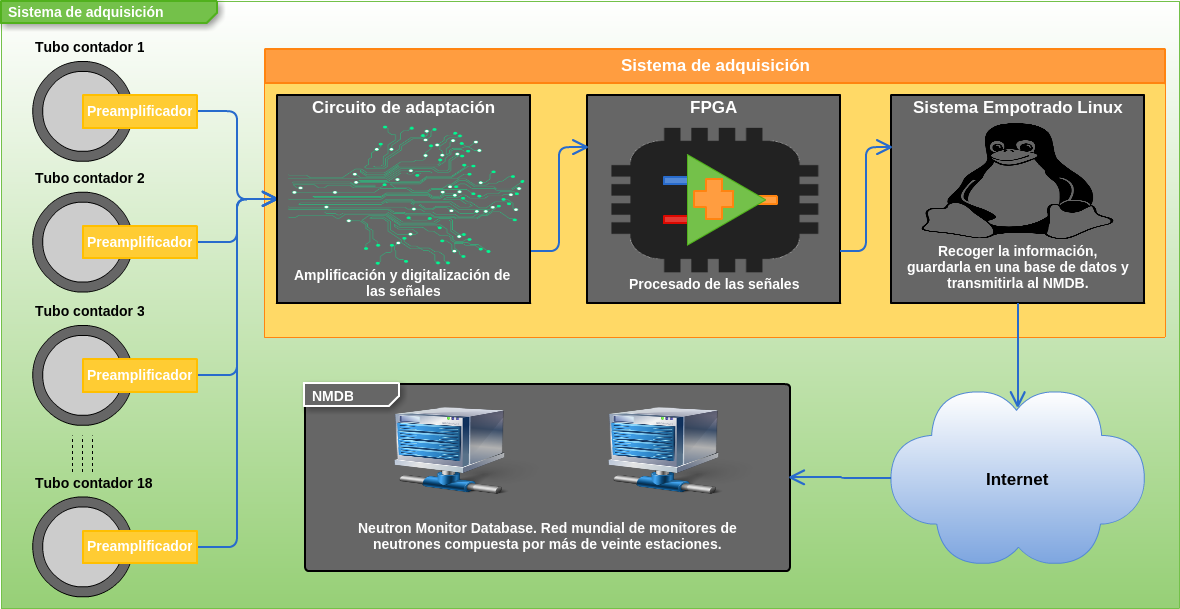
\includegraphics[keepaspectratio, width=1\textwidth]{./img/AcqSis.png}
			\caption{Sistema de adquisición.}
			\label{fig:acqsis}
		\end{figure}
		\par
		Actualmente el equipo de CALMA está desarrollando un nuevo sistema de adquisición de datos. Este es muy parecido al que actualmente
		está implantado. A continuación procedemos a detallar las diferencias clave entre los dos sistemas. 
		\par
		\begin{itemize}
			\item La primera diferencia entre los dos sistema de adquisición radica en el circuito de adaptación. En el sistema de
			  adquisición actual para cada señal el circuito de adaptación genera un pulso fijo. El nuevo sistema de adquisición incorpora
			  nuevo circuito de adaptación. Este nuevo circuito de adaptación genera un pulso cuyo ancho de banda es proporcional a la
			  energía de la señal. El fin es medir la energía de las partículas detectadas, esta magnitud es de gran interés científico y
			  técnico.
			\item La siguiente diferencia está en la FPGA, recordamos que en el sistema de adquisición actual esta tan solo registra los
			  eventos por minuto para los 18 canales. La nueva FPGA debe realizar la misma tarea, pero aparte debe poder medir el ancho de
			  los pulsos generados por el circuito de adaptación. Los dos sistemas de adquisición utilizan un puerto serie para la
			  comunicación entre software y FPGA, en el sistema nuevo este puerto opera a una velocidad mayor a fin de poder transmitir
			  toda la información extra.
			\item El nuevo sistema también está pensado para ofrecer una mayor compatibilidad. El fin es poder implantar este en
			  diferentes estaciones de forma fácil y rápida. El hardware y software deben ser diseñados con este requisito en mente.
		\end{itemize}
	\subsection{Bases de datos}
		La base de datos que genera CALMA está diseñada de acuerdo con el estándar impuesto por NMDB. Existen dos réplicas de la
		base de datos. Tenemos una réplica de los datos crudos adquiridos en el propio sistema, para gestionar esta réplica es utilizado
		Sqlite3. La segunda réplica está en otra máquina conectada por red con el sistema de adquisición de datos. Esta contiene los datos
		crudos y también contiene la corrección por presión de estos. Para la segunda réplica es utilizado MySQL. Los datos que son mandados
		al NMDB son los datos de la segunda réplica.
	\subsection{Herramientas y técnicas}
		El equipo de CALMA hace uso de herramientas que les ayudan a analizar la información desde el punto de vista científico. Actualmente
		no existe ninguna herramienta que proporcioné información sobre el estado técnico de la estación, todas las labores relacionadas con
		el mantenimiento son realizadas de forma manual.

\section{Objetivos}
	El objetivo de este proyecto es desarrollar el software para el nuevo sistema de adquisición de datos y también desarrollar una herramienta
	que permite operar y monitorizar el estado de la estación. A continuación procedemos a hacer una descripción más detallada de los objetivos de
	este trabajo.  
	\subsection{Software de adquisición}
		Tal y como hemos explicado en secciones anteriores el equipo de CALMA está desarrollando un nuevo sistema de adquisición. Actualmente
		la mayoría de módulos hardware incluyendo la FPGA están listos. El propósito de este trabajo es realizar el software de adquisición. A
		continuación exponemos algunos de los requisitos más relevantes.
		\begin{itemize}
			\item 	El software debe ser capaz de realizar una correcta comunicación con la FPGA. Esto implica enviar los comandos
				apropiados y ser capaz de interpretar los mensajes de datos trasmitidos por esta. En el capítulo \ref{entornoHW} se
				puede obtener más información sobre la interfaz de comunicación con la FPGA.
			\item 	El software debe ser capaz de mantener dos bases de datos, una réplica local y una remota.
			\item 	Al igual que el hardware, el software debe ser capaz de adaptarse fácilmente a diferentes estaciones. Para este
				propósito este debe ser diseñado de tal forma que sea fácil de extender.
			\item 	El software debe ser capaz de poner en marcha la estación completa de forma automática ante la presencia de corriente
			  	eléctrica. 
			\item 	El software debe ser capaz de detectar estados anómalos y actuar conforme a estos. En una estación de este tipo la
				mayoría de veces un funcionamiento anómalo se traduce en no generar datos o generar datos irregulares. Ante la
				presencia de un estado anómalo debe generarse una alarma. En muchos casos realizar un reinicio del sistema resuelve el
				problema.
		\end{itemize}
		Aparte de la realización del software en este trabajo también contemplamos el proceso de implantación y mantenimiento de este.
		Volvemos a recordar que los demás módulos que componen el sistema de adquisición son desarrollados por el equipo de CALMA. A lo largo
		de este trabajo se describirán las interfaces de estos, dado que es necesario para entender este trabajo.
	\subsection{Herramienta Web}
		El segundo objetivo de este trabajo es el desarrollo de una herramienta que facilite la gestión de una estación. La idea de esta
		herramienta es del equipo de CALMA. Procedemos a detallar las funcionalidades de la herramienta tal y como las concibe este.
		%TODO Citar el artículo de la herramienta.
		\begin{itemize}
			\item	Spike Tool. Módulo que permitirá la detección de Spikes. Usando los datos proporcionados por el sistema de
				adquisición, este módulo debe generar gráficos. Estos gráficos serán interactivos y su propósito será hacer fácil la
				detección de Spikes. Los Spikes detectados podrán ser marcados como nulos en el conjunto de datos revisados. El
				concepto de Spike es explicado en secciones venideras de este capítulo.
			\item 	Configuración de la estación. Este módulo permitirá cambiar la configuración de la estación. Esta reconfiguración será
				llevada a cabo en tiempo real sin interrumpir el proceso de adquisición. Nótese que el software de adquisición deberá
				evolucionar para hacer posible esta funcionalidad.
			\item	Alertas. La herramienta visualizará las alertas producidas por el software de adquisición.
			\item 	Histogramas con la intensidad de los eventos. El nuevo sistema de adquisición proporciona información sobre la energía
				de las partículas incidentes. Este módulo debería generar histogramas con estos datos. Estos histogramas permitirán
				hacer mejores diagnósticos sobre el funcionamiento de los tubos contadores. 
		\end{itemize}
		Podemos ver que la herramienta ofrece un gran abanico de funcionalidades. Por desgracia en este trabajo tan solo nos centraremos en el
		primer módulo, realizar los demás módulos está fuera del alcance de un trabajo como este. También cabe destacar que tan solo nos
		centraremos en la implementación, no implantaremos ni mantendremos la herramienta. La herramienta será una herramienta Web intuitiva y
		altamente interactiva.

\section{Diseño preliminar}
	En esta sección procedemos a especificar un diseño preliminar para el software de adquisición y para la herramienta Web.
	\subsection{Software de adquisición}
		El sistema de adquisición que se está desarrollando es un sistema empotrado donde hardware y software están muy vinculados. Esto en
		gran medida condiciona el diseño del software que queremos realizar. El software debe ejecutarse sobre una BeagleBone
		Black\cite{Beagle} que está integrada con el resto de componentes hardware.  La distribución Linux elegida para este trabajo es
		Angstrom. El lenguaje de programación elegido es Python\cite{Python}, lenguaje interpretado de alto nivel con tipado dinámico y
		sintaxis centrada en producir código legible.  Actualmente Python es muy popular y existen muchas librerías de las que haremos uso. El
		uso de librerías reduce la carga de trabajo y normalmente resulta en software más robusto. Para la gestión de la base de datos hemos
		elegido Sqlite3\cite{Sqlite}, una elección popular en sistemas empotrados. 
		\par
		En la figura \ref{fig:soft_control_preliminar} podemos ver el diseño preliminar del software de adquisición. Ante la presencia de
		corriente eléctrica este debe ser capaz de inicializarse solo. El primer paso que debe tomar es realizar la configuración necesaria
		para el correcto funcionamiento del sistema de adquisición. Seguidamente debe continuar con el funcionamiento nominal. Este consiste
		de tres pasos que se repiten cíclicamente. El primero es solicitar la información a la FPGA, seguidamente el software debe interpretar
		dicha información y finalmente la información debe ser guardada. Los posibles estados anómalos deben ser detectados y contrarrestados. 
		\begin{figure}[h]
			\centering
			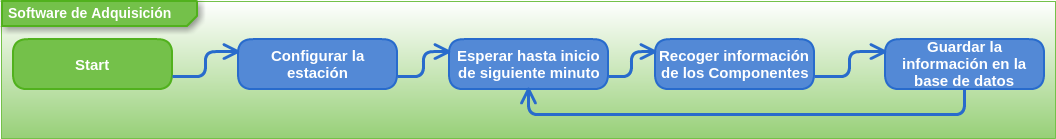
\includegraphics[keepaspectratio, width=1\textwidth]{./img/soft_control_preliminar.png}
			\caption{Software de adquisición. Diseño preliminar.}
			\label{fig:soft_control_preliminar}
		\end{figure}
	\subsection{Herramienta Web}
		En la figura \ref{fig:herramienta_web_preliminar} podemos ver el diseño preliminar de la herramienta Web. Como podemos ver el diseño
		está fuertemente basado en el patrón \emph{Modelo Vista Controlador}\cite{MVCWiki}. A continuación explicamos los tres componentes
		básicos.
		\begin{description}
			\item[Base de Datos]    
				En este componente residen los datos de nuestra estación. Para la gestión de estos utilizamos un servidor
				MySQL\cite{MySql}.
			\item[\emph{Back-End}]
				Este componente es el encargado de recibir y procesar los mensajes de petición provenientes del \emph{Front-End}.
				Estas peticiones pueden ser de consulta o de acción. En ambos casos este componente procede a comunicarse con la base
				de datos a fin de satisfacer la petición. Finalmente el resultado es trasmitido al \emph{Front-End} en un mensaje de
				respuesta. En el caso de una petición de consulta son devueltos los datos especificados. En el caso de una petición de
				acción es devuelto un mensaje de estado. Para la implementación de este componente hemos utilizado
				ZendFramework\cite{ZF} y Apygility\cite{Apigility}.
			\item[\emph{Front-end}] 
				Este componente implementa la interfaz de nuestra aplicación. Es el encargado de presentar la información y manejar
				las peticiones del usuario. El módulo está basado en el patrón MVC. Para implementar la Vista hemos utilizado
				HighStock\cite{HighStock}, para el Controlador ExtJs\cite{ExtJs} y para el modelo peticiones Ajax\cite{AjaxWiki}.
		\end{description}
		\begin{figure}[h]
			\centering
			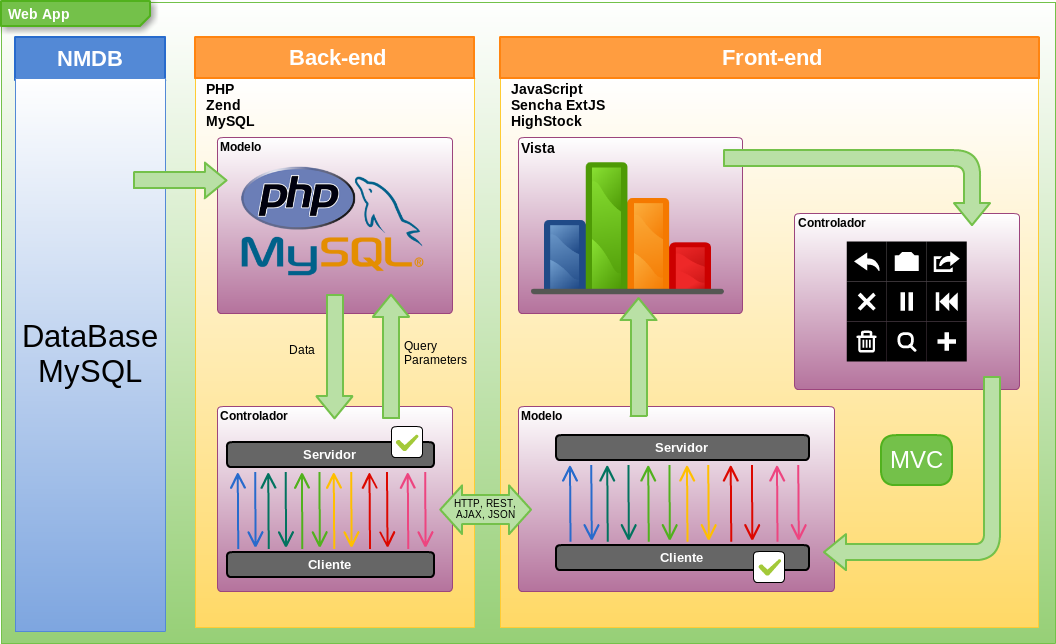
\includegraphics[keepaspectratio, width=1\textwidth]{./img/herramienta_web_preliminar.png}
			\caption{Herramienta Web. Diseño preliminar}
			\label{fig:herramienta_web_preliminar}
		\end{figure}
\section{Proceso de adquisición}
	El propósito de este punto es explicar algunos aspectos del proceso de adquisición que son relevantes para este trabajo.
	\begin{description}[leftmargin=0cm]
		\item[Múltiples Tubos]
			Hasta este momento siempre hemos hablado de tubos contadores, en plural, detrás de esto hay una razón. Normalmente las
			estaciones se componen de varios tubos contadores, donde 18 tubos contadores es un estándar. En el proceso de adquisición
			están envueltos muchos factores probabilísticos, esto conlleva a que las medidas en un tubo tengan una gran dispersión. La
			solución de este problema es tener mucho tubos, cuantos más mejor. Combinando datos de diferentes tubos conseguimos reducir
			esta dispersión. 
		\item[Valor global]
		  	Tener los datos de muchos tubos contadores permite reducir la dispersión de los datos, sin embargo no es muy práctico trabajar
			con esos datos en crudo. El software del sistema de adquisición actual calcula un valor global a partir de los datos de todos
			los tubos contadores. El software de adquisición que desarrollamos en este trabajo también debe calcular este valor global.
			Para este propósito utilizamos el Median Algorithm\cite{MedianAlgr}.
		\item[Correcciónes]
			Anteriormente en este capítulo explicamos las cascadas atmosféricas que son originadas por los rayos cósmicos. Estas cascadas
			atmosféricas dependen de la presión atmosférica. Cuando esta es elevada, es necesaria más energía para que la cascada se
			propague hasta el nivel terrestre, por consecuente los monitores de neutrones registran menos eventos. El valor de la presión
			atmosférica es monitorizado por los monitores de neutrones. Este valor es utilizado para realizar una corrección por presión
			sobre el valor global de la estación, a lo largo de este trabajo utilizamos el término de \emph{valor corregido por presión}
			para referirnos a este valor. El software de adquisición elaborado para este trabajo debe ser capaz de leer el valor de
			presión desde un barómetro y debe poder calcular esta corrección. 
			\par
			También es realizada una \emph{corrección por eficiencia}. Esta es muy simple y consiste en aplicar un factor multiplicativo
			al valor corregido por presión. Este valor es utilizado para para solventar problemas técnicos. Cambios en el entorno
			inmediato del instrumento o cambios en la electrónica utilizada pueden afectan a la cantidad de eventos medidos. Estos cambios
			son identificados, evaluados y finalmente contrarrestados con esta corrección por eficiencia. Este valor dota la estación de
			consistencia histórica, de esta manera pueden ser comparados datos de diferentes intervalos temporales. El software también
			debe ser capaz de realizar esta corrección. 
		\item[Fuentes de alta tensión]
			A principios de este capítulo explicamos que los tubos contadores están rellenos de gas ionizado. Este gas es ionizado
			mediante la aplicación de una corriente eléctrica de alta tensión. Para la generación de esta corriente son utilizadas fuentes
			de alimentación de alta tensión. Cambios en la corriente generada pueden afectar a la cantidad de eventos registrados. Esto ha
			conllevado a que el funcionamiento de las fuentes sea monitorizado. El software para el sistema de adquisición debe ser capaz
			de realizas esta operación. Es de esperar que la corriente sea constante, por lo que no es necesaria ninguna corrección en
			función de esta. En caso de variaciones en la corriente los datos generados son considerados no consistentes.
		\item[\emph{Spikes}]
			Un \emph{Spike} es un dato anómalo, un dato anormalmente grande o pequeño. Son datos producidos por malfuncionamientos de la
			instrumentación, cambios bruscos en el entorno inmediato u otros factores desconocidos. Estos están presentes en todas las
			estaciones. Con la elaboración del nuevo sistema de adquisición se pretende reducir el número de \emph{Spikes} generados. Con
			la elaboración de la herramienta Web pretendemos ofrecer un método fácil de identificar y descartar dichos datos.
	\end{description}

\chapter{Entrono Hardware}
\label{entornoHW}

En un sistema empotrado el software y hardware están muy vinculados. Para entender el funcionamiento del software de adquisición es muy importante estar
familiarizado con el diseño y funcionalidad del hardware. Impulsados por esta razón en este capítulo procederemos a hacer una descripción de
los aspectos más importantes del hardware que compone nuestro sistema de adquisición. Volvemos a enfatizar que el autor de este trabajo no
ha formado parte  en la realización de los módulos hardware que serán descritos a continuación.
\section{BeagleBone Black}
	BeagleBone Black\cite{Beagle}\cite{BeagleWiki} es un computador empotrado, open-source y single board. La placa viene con Linux, distribución Angstrom y versión
	de núcleo 3.8. En la figura \ref{fig:beaglebone} podemos ver un diagrama de bloques que refleja los componentes hardware que componen la
	BeagleBone. A continuación vamos a hacer una breve descripción de los módulos que utilizaremos para este trabajo.
	\begin{itemize}
	  \item 	ARM CORTEX A8\cite{BeagleCore} y SDRAM. El procesador es suficientemente potente para soportar la distribución Linux y satisfacer
	    		las necesidades de nuestro software. Los 512MB DDR3 de memoria RAM son suficientes para los propósitos de este trabajo.
		\item 	Ethernet Connector. El conector RJ-45 nos permitirá conectarnos a Internet. Una vez establecida la conexión podremos transmitir
		  	los datos al NMDB. La conexión también nos permitirá conectarnos a la placa vía SSH, de esta manera un operador podría realizar
			operaciones de mantenimiento de forma remota. 
		\item	eMMC y microSD. Utilizaremos la memoria integrada (eMMC) de 4GB para albergar el sistema operativo y el software de adquisición.
		  	La microSD la utilizaremos para guardar los datos y logs producidos por el software de adquisición.
		\item 	Analog Pins. Los 7 pines analógicos nos permiten usar sensores cuyo output es una señal analógica. Ejemplo de estos sensores son
		  	las fuentes de alimentación analógicas o los sensores de temperatura, en algunas estaciones la temperatura ambiente se monitoriza
			también. Estos sensores producen señales cuya tensión eléctrica es proporcional al valor de la magnitud medida. 
		\item 	GPIOs. Las GPIO nos permiten trabajar con señales digitales, tanto de entrada como de salida. Un ejemplo de uso es la señal de
		  	Reset de la FPGA, señal digital activa a bajo nivel.
		\item	UARTs. La placa ofrece 4 puertos series de los que utilizaremos 2 para comunicarnos con la FPGA.
	\end{itemize}
	\begin{figure}[h]
		\centering
		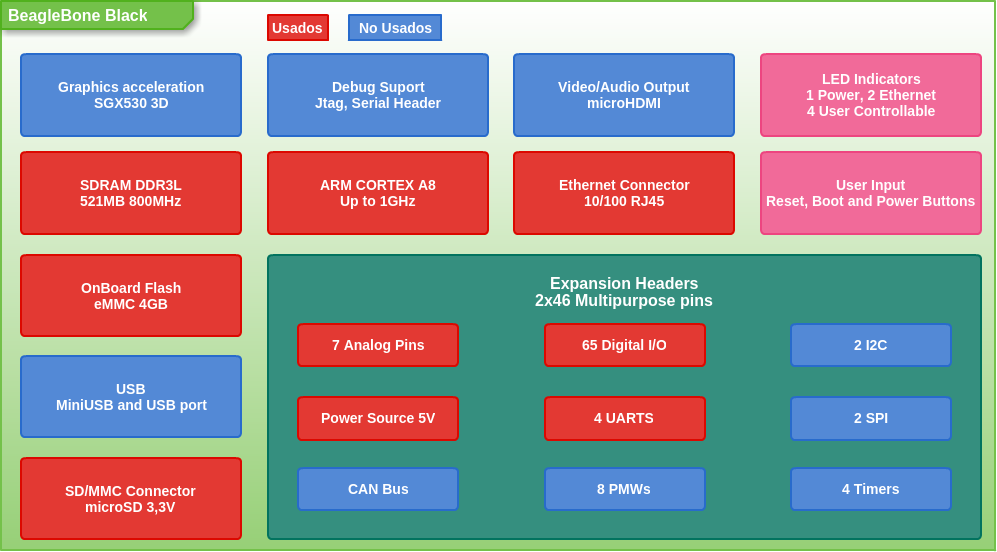
\includegraphics[keepaspectratio, width=1\textwidth]{./img/beaglebone.png}
		\caption{BeagleBone Black. Diagrama de bloques hardware}
		\label{fig:beaglebone}
	\end{figure}
	Fijándonos en la figura \ref{fig:beaglebone} podemos ver que muchos de los módulos son accesibles mediante los pines de extensión\cite{BeagleWikiExp}.
	La placa ofrece 2x46 pines de los cuales muchos son multipropósito, pueden ser configurados para tener funcionalidades diversas y además esta
	configuración puede ser realizada de forma dinámica. La configuración de los pines se realiza mediante el \emph{Device Tree Overlay}, estructura de
	datos que se utiliza para describir el hardware. Para la realización de este trabajo no tendremos que lidiar con este mecanismo, utilizaremos una
	librería que nos facilite el trabajo. La librería utilizada es \emph{Adafruit BeagleBone IO Python}\cite{AdaFruitGit}. Esta librería nos ayudara a
      	configurar dinámicamente los pines de extensión, además la librería ofrece métodos para operar sobre estos una vez configurados.


\section{FPGA}
	En esta sección vamos a hacer una descripción de la FPGA. En la figura \ref{fig:fpga} podemos ver un diagrama de bloques que refleja los módulos
	funcionales y las interfaces que posee la FPGA.
	\begin{figure}[h]
		\centering
		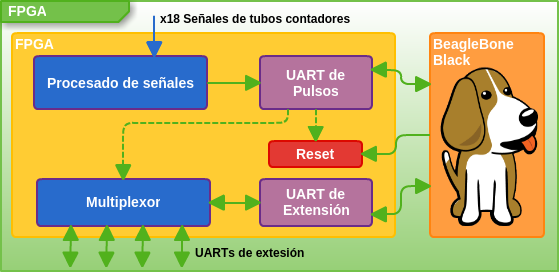
\includegraphics[keepaspectratio, width=1\textwidth]{./img/fpga.png}
		\caption{FPGA. Diagrama de bloques.}
		\label{fig:fpga}
	\end{figure}	
	\subsection{Procesado de pulsos}
		Como ya hemos comentado en el capítulo \ref{cap1} la FPGA se encarga de procesar las señales provenientes de los tubos, una vez procesadas
		las señales, la información es transmitida a la BeagleBone Black. Esta transmisión se realiza mediante una UART a la que nos referiremos
		como UART de pulsos. En las tablas \ref{tab:FPGAUartPulso}, \ref{tab:FPGAUartOver}, \ref{tab:FPGAUartCont} podemos ver el formato de los
		datos transmitidos. Vemos que hay tres diferentes mensajes que la FPGA nos puede transmitir.
		\begin{itemize}
			\item	En la tabla \ref{tab:FPGAUartPulso} podemos ver el formato del primer mensaje que vamos a discutir. Este mensaje se
			  	constituye de tres bytes que nos dan información sobre el ancho de un pulso. El mensaje nos permite identificar el canal
				en el que se ha producido el pulso, el nivel (alto/bajo) y la longitud de este. Los pulsos de nivel alto representan la
				detección de una partícula por los tubos contadores, el ancho del pulso es proporcional a la energía de la partícula
				detectada. La longitud de los pulsos de nivel bajo también es mediada para poder identificar pulsos con pequeña
				separación temporal.
			\item 	En la siguiente tabla \ref{tab:FPGAUartOver} podemos ver el mensaje de estado que la FPGA genera. Dado que la UART usa
			  	una FIFO de tamaño fijo es posible que la FIFO se llene y se pierdan mensajes. En este caso la FPGA genera un mensaje de
				estado que es transmitido para indicarle al software que se han producido perdidas de datos.
			\item	Además de medir el ancho de los pulsos la PFGA lleva la cuenta de pulsos recibidos para cada canal. Esta información
			  	puede ser solicitada por la BeagleBone Black utilizando el comando apropiado, ver tabla \ref{tab:FPGAUartComm}. En la
				tabla \ref{tab:FPGAUartCont} podemos ver el formato en el que se transmite la información de las cuentas. Los bytes
				2, 3, 4 son transmitidos 18 veces, una vez para cada canal. Después de transmitir la información de las cuentas la FPGA
				reinicia los contadores para cada canal.
		\end{itemize}
		En la figura \ref{fig:fpgaWave} podemos ver un posible diagrama de como se generan los mensajes anteriormente descritos.

		\begin{table}[h]
			\tiny
			\begin{tabularx}{\textwidth}{|l|c|c|X|c|c|c|c|c|}
				\hline
				\rowcolor[HTML]{C0C0C0} 
				\multicolumn{1}{|r|}{\textbf{Bit}}    	& 7 & 6          & 5 				& 4 	       & 3 	     & 2 	  & 1          & 0 	     \\ \hline
				\cellcolor[HTML]{C0C0C0}\textbf{Byte 1} & 0 & 1          & 0  				& \multicolumn{5}{c|}{Canal (0-17)}				     \\ \hline
				\cellcolor[HTML]{C0C0C0}\textbf{Byte 2} & 1 & Dato (6)	 & Dato (5)      		& Dato (4)     & Dato (3)    & Dato (2)   & Dato (1)   & Dato (0)    \\ \hline
				\cellcolor[HTML]{C0C0C0}\textbf{Byte 3} & 1 & X          & Nivel ('1'->alto, '0'->bajo) & Dato (11)    & Dato (10)   & Dato (9)   & Dato (8)   & Dato (7)    \\ \hline
			\end{tabularx}
			\caption{UART pulsos. Palabra de ancho de pulso}
			\label{tab:FPGAUartPulso}
			\begin{tabularx}{\textwidth}{|l|c|X|X|X|X|X|X|X|}
				\hline
				\rowcolor[HTML]{C0C0C0} 
				\multicolumn{1}{|r|}{\textbf{Bit}} 	& 7 & 6 		       & 5 		       & 4		       & 3 		       & 2		       & 1          	       & 0			\\ \hline
				\cellcolor[HTML]{C0C0C0}\textbf{Byte 1} & 0 & 0                        & OverFlow FIFO Tubo 5  & OverFlow FIFO Tubo 4  & OverFlow FIFO Tubo 3  & OverFlow FIFO Tubo 2  & OverFlow FIFO Tubo 1  & OverFlow FIFO Tubo 0	\\ \hline
				\cellcolor[HTML]{C0C0C0}\textbf{Byte 2} & 1 & OverFlow FIFO Tubo 12    & OverFlow FIFO Tubo 11 & OverFlow FIFO Tubo 10 & OverFlow FIFO Tubo 9  & OverFlow FIFO Tubo 8  & OverFlow FIFO Tubo 7  & OverFlow FIFO Tubo 6	\\ \hline
				\cellcolor[HTML]{C0C0C0}\textbf{Byte 3} & 1 & Almost Full FIFO General & OverFlow FIFO General & OverFlow FIFO Tubo 17 & OverFlow FIFO Tubo 16 & OverFlow FIFO Tubo 15 & OverFlow FIFO Tubo 14 & OverFlow FIFO Tubo 13	\\ \hline
			\end{tabularx}
			\caption{UART pulsos. Palabra de estado}
			\label{tab:FPGAUartOver}
			\begin{tabularx}{\textwidth}{|l|X|c|c|c|c|c|c|c|}
				\hline
				\rowcolor[HTML]{C0C0C0} 
				\multicolumn{1}{|r|}{\textbf{Bit}}    	 & 7 & 6           & 5 		& 4 	      & 3 	    & 2 	 & 1           & 0 	     	\\ \hline
				\cellcolor[HTML]{C0C0C0}\textbf{Byte 1}  & 0 & 1           & 1  	& X	      & X	    & X	  	 & X	       & X	     	\\ \hline
				\cellcolor[HTML]{C0C0C0}\textbf{Byte 2}  & 1 & Dato0 (6)   & Dato0 (5) 	& Dato0 (4)   & Dato0 (3)   & Dato0 (2)  & Dato0 (1)   & Dato0 (0)  	\\ \hline
				\cellcolor[HTML]{C0C0C0}\textbf{Byte 3}  & 1 & Dato0 (13)  & Dato0 (12)	& Dato0 (11)  & Dato0 (10)  & Dato0 (9)  & Dato0 (8)   & Dato0 (7)  	\\ \hline
				\cellcolor[HTML]{C0C0C0}\textbf{Byte 4}  & 1 & X	   & X	 	& X	      & X	    & X		 & Dato0 (15)  & Dato0 (14)	\\ \hline
				\cellcolor[HTML]{C0C0C0}\textbf{Byte 5}  & 1 & Dato1 (6)   & Dato1 (5) 	& Dato1 (4)   & Dato1 (3)   & Dato1 (2)  & Dato1 (1)   & Dato1 (0)  	\\ \hline
				\cellcolor[HTML]{C0C0C0}\textbf{......}  & . & .........   & ......... 	& .........   & .........   & .........  & .........   & .........  	\\ \hline
				\cellcolor[HTML]{C0C0C0}\textbf{Byte 55} & 1 & X	   & X	 	& X	      & X	    & X		 & Dato17 (15) & Dato17 (14)	\\ \hline
			\end{tabularx}
			\caption{UART pulsos. Palabra de cuentas}
			\label{tab:FPGAUartCont}
			\begin{tabularx}{\hsize}{|c|X|}
		  		\hline
				\rowcolor[HTML]{C0C0C0} 
		  		Commando & Descripción                            \\\hline
		  		0x00     & Configura multiplexor para aparato 1   \\\hline
		  		0x01     & Configura multiplexor para aparato 2   \\\hline
		  		0x02     & Configura multiplexor para aparato 3   \\\hline
		  		0x03     & Configura multiplexor para aparato 4   \\\hline
		  		0x10     & Reset general del sistema              \\\hline
		  		0x11     & Solicita la transmisión de las cuentas \\\hline
			\end{tabularx}
			\caption{UART pulsos. Commandos}
			\label{tab:FPGAUartComm}
		\end{table}
		\begin{figure}[h]
			\centering
			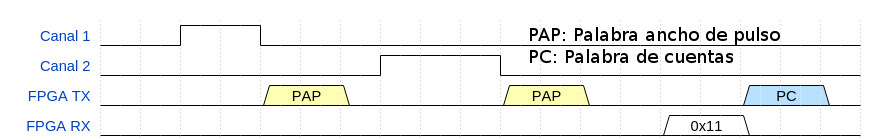
\includegraphics[keepaspectratio, width=1\textwidth]{./img/fpgawave.png}
			\caption{FPGA. Diagrama de eventos.}
			\label{fig:fpgaWave}
		\end{figure}
	\subsection{Multiplexor}
		Entre la FPGA y la BeagleBone Black hay una segunda UART a la que nos referiremos como UART de extensión. Esta UART tiene como propósito
		extender el número de UART que podemos conectar a nuestro sistema. La UART de extensión está conectada a un multiplexor implementado en la
		FPGA. El multiplexor tiene como entradas 4 UARTs. Podemos seleccionar una entrada diferente mandando comandos a la FPGA por la UART de pulsos,
		de acuerdo a la especificación de la tabla \ref{tab:FPGAUartComm}. Esta extensión nos permite conectar más sensores que requieran una UART.
		Un ejemplo es el barómetro \emph{BM35}\cite{BM35} utilizado en CALMA.
	\subsection{Reset}
		La FPGA nos permite realizar un Reset del sistema. Todas las variables son puestas a sus valores iniciales, excepto el multiplexor que mantiene
		su estado. Existen dos maneras de realizar este Reset. La primera es mediante un comando trasmitido por la UART de  pulsos, de acuerdo a la
		especificación presentada en la tabla \ref{tab:FPGAUartComm}. La segunda manera de realizar este Reset es mediante una señal digital activa a
		bajo nivel. La señal mencionada está conectada a la BeagleBone Black por lo que es posible realizar el Reset desde nuestro software de adquisición. 

\chapter{Software de adquisición}
\label{cap2}
En este capítulo procedemos a explicar el funcionamiento del software de adquisición. Empezaremos recordando los aspectos básicos descritos en el
capítulo de introducción. El funcionamiento nominal del software consiste en recoger la información de los módulos hardware como la FPGA, el
barómetro, las fuentes de alimentación y los sensores de temperatura si estos están presentes. Cada minuto la información recogida es procesada y
almacenada en una base de datos. 
\par
Antes de empezar a discutir a fondo el software de adquisición es conveniente estar familiarizados con el entorno hardware descrito en el capítulo
\ref{entornoHW}. El software es ejecutado en la BeagleBone Black sobre un Linux, distribución Angstrom. El lenguaje elegido para el desarrollo es
Python\cite{Python}. Este  es un lenguaje interpretado de alto nivel con una sintaxis centrada en producir un código legible. El lenguaje se adapta
igualmente bien a programación imperativa y orientada a objetos. El tipado dinámico da mucha flexibilidad al lenguaje. Todas estas propiedades del
lenguaje permiten un desarrollo rápido. Además el lenguaje ofrece una amplia cantidad de librerías que también aligeran el trabajo. 
\par
Para gestionar la base de datos utilizamos Sqlite3\cite{Sqlite}. Este es un gestor muy ligero y adecuado para sistemas empotrados. Aparte de esta base
de datos local el software permite mantener una segunda réplica remota. Para esta réplica remota utilizamos MySql\cite{MySql} que es un gestor más
completo con enfoque \emph{Cliente-Servidor}.
\par
En la figura \ref{fig:soft_adquisición} podemos ver un diagrama de flujo que describe el funcionamiento de nuestro software. A lo largo de este
capítulo haremos muchas referencias a este diagrama para explicar los diferentes módulos software que lo componen. Podemos ver que hay cuatro módulos
principales, a continuación hacemos una breve descripción de estos. 
\begin{itemize}
  	\item	\texttt{NMDA}. Es el proceso principal de nuestro software. Este es el encargado de realizar las configuraciones necesarias e iniciar
	  	el \texttt{FPGASerialReader} y el \texttt{CountsManager}.
	\item	\texttt{FPGASerialReader}. Thread que se encarga de procesar la información transmitida por la FPGA.
	\item	\texttt{CountsManager}. Thread que se enarga de pedir la información necesaria y guardarla en la base de datos con periodicidad de un
	  	minuto. Después de guardar la información es iniciado el \texttt{DBUpdater}.
	\item	\texttt{DBUpdater}. Thread que se encarga de sincronizar la base de datos local con la réplica remota.
\end{itemize}

\begin{sidewaysfigure}[p]
	\centering
	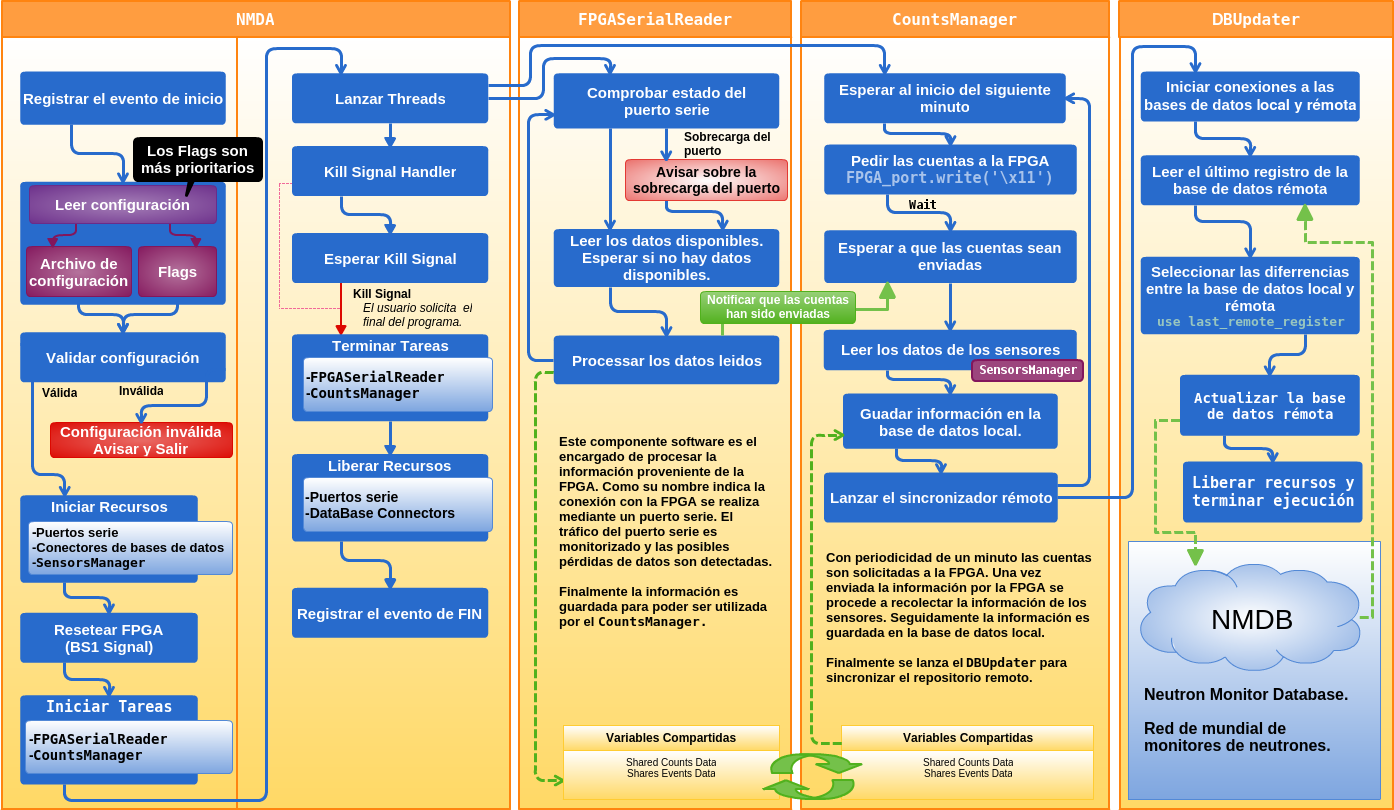
\includegraphics[keepaspectratio, width=1\textwidth]{./img/soft_adquisicion.png}
	\caption{Diagrama de flujo. Software de adquisición.}
	\label{fig:soft_adquisición}
\end{sidewaysfigure}

\section{Arranque automático del sistema}
	Uno de los requisitos del sistema es el arranque automático ante la presencia de corriente eléctrica. La BeagleBone Black por defecto está
	configurada para arrancar automáticamente, debemos configurarla para que inicialice nuestro software. Para este propósito vamos a utilizar las
	\emph{System Services}\cite{AngSystemctl} que Angstrom proporciona. Un servicio de sistema permite ejecutar un programa de forma automática al
	ser arrancado el sistema. Angstrom utiliza \texttt{systemd}\cite{systemdWiki} para gestionar los servicios de sistema.  Este es un conjunto de
	demonios, librerías y utilidades diseñados para facilitar la administración de sistemas Linux.
	\par
	Para operar sobre la configuración de \texttt{systemd} tenemos el comando \texttt{systemctl}. A continuación podemos ver como usar este
	comando.
	\begin{lstlisting}[style=myBash]
$ systemctl start    nombre_de_servicio
$ systemctl restart  nombre_de_servicio
$ systemctl stop     nombre_de_servicio
$ systemctl status   nombre_de_servicio
$ systemctl enable   nombre_de_servicio
$ systemctl disable  nombre_de_servicio
	\end{lstlisting}
	\par
	Los servicios de sistema se crean mediante archivos con extensión \texttt{.service} que deben ser guardados en el directorio
	\texttt{/lib/systemd/system}. En el apéndice \ref{appendix:systemctl} podemos ver el contenido de los archivos que definen los cuatro
	servicios de sistema utilizados en este trabajo. Veamos el significado de lo campos más importantes que son definidos en estos archivos.
	\begin{itemize}
		\item	\texttt{Description}. Un mensaje descriptivo del servicio. Permite al usuario entender el propósito de este de forma fácil.
		\item	\texttt{Before} y \texttt{After}. Estos dos campos pueden referenciar a otros servicios para indicar que este debe ejecutarse
			antes o después del servicio que es citado. Esto permite definir un orden en el que serán ejecutados los servicios de sistema.
			También es posible especificar un grupo de servicios como el \texttt{network.target} que agrupa los servicios responsables de
			establecer la conexión a Internet. 
		\item	\texttt{Type}. El tipo del servicio. Con este campo podemos dar diferentes propiedades a nuestro servicio. Los valores
			aceptados que utilizamos son \texttt{oneshot}, \texttt{forking} y \texttt{simple}, que es el valor por defecto.
		\item	\texttt{ExecStart}. El comando y argumentos que queremos ejecutar.
		\item	\texttt{WantedBy}. Es el grupo al que este servicio pertenece. El grupo \texttt{multi-user.target} es un grupo para los
			servicios de un sistema multiusuario. Este campo hace que este servicio sea retrasado hacia el final del proceso de arranque,
			específicamente hasta que el sistema sea listo para aceptar el acceso de múltiples usuarios. 
	\end{itemize}
	\par
	En la figura \ref{fig:boot} podemos ver la secuencia que define el proceso de arranque del sistema de adquisición. Para cumplir con este
	proceso hemos definido cuatro servicios de sistema. El servicio \texttt{myWatchDog.service} es el encargado de arrancar el software que
	controla el Watchdog. El servicio \texttt{ntpdate.service} es el responsable de actualizar la fecha y hora actuales. El servicio
	\texttt{ntpd.service} es el responsable de mantener sincronizados la fecha y hora del sistema. Finalmente el servicio \texttt{nmda.service} es
	el encargado de arrancar el software de adquisición.
	\begin{figure}[h]
		\centering
		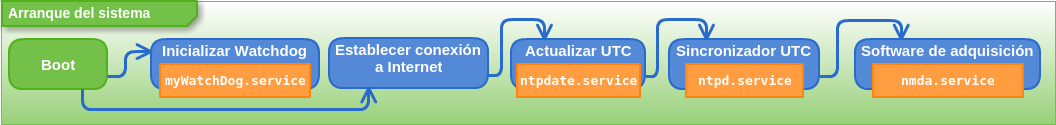
\includegraphics[keepaspectratio, width=1\textwidth]{./img/boot.png}
		\caption{Arranque del sistema}   
		\label{fig:boot}
	\end{figure}
	\subsection{Watchdog}
		Un Watchdog \cite{WatchDogWiki} es un mecanismo de seguridad que realiza un Reset en el sistema cuando es detectado un
		mal funcionamiento. Consiste en un temporizador que realiza una cuenta atrás, cuando esta cuenta llega a cero el sistema es reiniciado.
		Es nuestro software el que debe reiniciar este contador para que no expire. Los Watchdogs pueden ser software o hardware, el utilizado
		en este trabajo está implementado en la BeagleBone Black y es hardware. Los Watchdogs hardware son más fiables, los software pueden
		quedarse bloqueados.
		\par
		El Watchdog es accesible mediante el archivo \texttt{/dev/watchdog}. Para activar el mecanismo escribimos en el archivo, cualquier
		valor es aceptado. El contador es puesto en marcha, si este llega a expirar es reiniciada la placa. El valor inicial del contador es
		de 60 segundos, valor que adquiere cada vez que es reiniciado. El contador es reiniciado al escribir en el archivo. Al cerrar dicho
		archivo el mecanismo es deshabilitado. A continuación presentamos una parte del código fuente responsable de controlar el WatchDog.
		\begin{lstlisting}[style=myPython]
args		= NMDA.create_parser().parse_args()
conn_local      = sqlite3.connect(args.database)
last_data       = get_last()
cont            = 0

wd = open("/dev/watchdog", "w+")
while True:
    time.sleep(20)
    wd.write("\n")
    wd.flush()
    cont+=1

    if cont >= 15:            #15*20secs=5mins
        cont            = 0
        curr_last       = get_last()
        if curr_last == last_data:
            time.sleep(120)   #Este sleep reinicia la placa
        last_data       = curr_last
		\end{lstlisting}
		\par
		Primero se establece la conexión con la base de datos local. La base de datos es utilizada para comprobar si el sistema de adquisición
		genera correctamente datos, si no son generados datos la placa debe ser reiniciada. Una vez establecida la conexión se procede a
		invocar la función \texttt{get\_last()}, que devuelve el último valor presente en la base de datos. Seguidamente es abierto el archivo
		que permite manejar el WatchDog. Una vez abierto el archivo se entra en un bucle \texttt{while} sin condición de salida. En cada
		iteración de este bucle es escrito un salto de línea que reinicia el contador del WatchDog. Dentro del bucle también hay una llamada a
		la función \texttt{time.sleep(20)}, las iteraciones del bucle están espaciadas 20 segundos. Cada 15 iteraciones o aproximadamente 5
		minutos se vuelve a invocar la función \texttt{get\_last()}. El valor devuelto es comparado con el valor anterior. Si estos dos
		valores son iguales es invocada la función \texttt{time.sleep(120)}, intervalo suficiente para que el contador del WatchDog expire.
		Los valores son iguales si en los últimos 5 minutos el sistema de adquisición no ha generado ningún dato. Por contrario si se han
		generado datos durante los últimos 5 minutos estos dos valores son diferentes, en tal caso se sigue con la ejecución del bucle
		\texttt{while}. 
	\subsection{Sincronización UTC}
		La BeagleBone Black no implementa ningún mecanismo hardware para calcular la fecha y hora actuales, por lo que en cada reinicio la
		fecha y hora se pierden. Es nuestra responsabilidad realizar un mecanismo software que sincronice la fecha y hora con el resto del
		mundo\cite{ntpd}. Es utilizado el programa \texttt{ntpd} para este propósito. Este es un programa que hace uso del \emph{Network Time
		Protocol}\cite{ntpWiki} para mantener el tiempo del sistema. Son realizadas dos llamadas a este programa.
		\begin{lstlisting}[style=myBash]
# Actualiza la fecha y hora.
$ /usr/bin/ntpd -q -g -x
# Lanza un demonio que corrige las derivas que puedan presentarse
$ /usr/bin/ntpd -p /run/ntpd.pid
		\end{lstlisting}

\section{\texttt{NMDA}}
	Este es el módulo principal de nuestro software. En la figura \ref{fig:soft_adquisición} podemos ver un diagrama de flujo que representa el
	funcionamiento de este. En las siguientes subsecciones describiremos las funcionalidades más relevantes de este módulo.
	\subsection{Logger}
		Haciendo uso de la librería \texttt{logging}\cite{py_logging} es configurado un archivo de Log. En este archivo son registrando los
		sucesos de eventos importantes. Ejemplo de eventos que registramos son las pérdidas de datos o el inicio del sistema. El mecanismo
		está configurado para que automáticamente se guarde la hora y fecha de cada mensaje. A continuación se muestra como se configura y usa
		este mecanismo.
		\begin{lstlisting}[style=myPython]
import logging
logging.basicConfig(filename='/server/logs/NMDA.log', level=logging.DEBUG, format=''%(asctime)s %(message)s'')
logging.info('Started')
		\end{lstlisting}
	\subsection{Archivo de configuración y Flags}
		Existen una serie de variables que varían en función de la estación o que simplemente pueden cambiar con el tiempo. No es buena idea
		tener los valores de estas variables en el código. Este problema nos ha llevado a exportar estas variables a un archivo de
		configuración.  Para leer este archivo utilizamos la librería \texttt{ConfigParser}\cite{py_ConfigParser}. A continuación mostramos un
		ejemplo de este archivo que nos ayudara a entender mejor su estructura.
		\begin{lstlisting}[style=myFile]
[Basics]
# The serial RS232_FPGA1C
serial_port_control  = /dev/ttyO2
# The local database where data will be saved. If 'shell' is specified as database data will be printed to the shell
database = /server/data/test.db
# Channel averages used for the median algorithm\ldots
Channel_avg = 255, 290, 0, 295, 0, 0, 289, 291, 252, 254, 293, 299, 298, 328, 299, 302, 302, 272

[Sensors]
# The serial RS232_FPGA1
serial_port_sensors= None
# The type of barometer that will be used. 'None', 'bm35', 'ap1'
barometer_type = None
# The type of hvps that will be used. 'None', 'analog', 'digital'
hvps_type = None
#Correction coefficient for the analog hvps, 1.0 => No correction
analog_hvps_corr = 1.0

[dbUpdater]
db_updater_enabled=True
# Must be the same that Basic.database
local_db= /server/data/test.db 
# The remote database config
remote_db_host= 192.168.1.1
# The user must have privileges
remote_db_user= hristo
remote_db_pass= 123qwe
# The database will be created if not exists along with all the tables
remote_db_db= nmdadb2

[Pressure]
# Average pressure for the station.
avg_pressure=932
# N=N0*exp(Beta*(P-P0))
beta_pressure=0.0067

[Efficiency]
# corr_efficcincy = Beta * corr_pressure
beta_efficiency=1.0
\end{lstlisting}
		Los valores de las variables exportadas son también accesibles mediante el uso de Flags. En este caso hemos utilizado la librería
		\texttt{argparse}\cite{py_argparse}. Los valores que son especificados con Flags sobrescriben a los valores del archivo de
		configuración. Los Flags se usan de la siguiente forma.
		\begin{lstlisting}[style=myBash]
$ python NMDA.py -h
usage: NMDA.py 
   [-h] [-sp SERIAL_PORT_CONTROL] [-db DATABASE]
   [-sps SERIAL_PORT_SENSORS] [-bm {ap1,bm35}]
   [-hv {digital,analog}] [-ahvc ANALOG_HVPS_CORR]
   [-dbU DB_UPDATER_ENABLED] [-ldb LOCAL_DB] [-rh REMOTE_DB_HOST]
   [-ru REMOTE_DB_USER] [-rp REMOTE_DB_PASS] [-rdb REMOTE_DB_DB]
   [-apr AVG_PRESSURE]
		\end{lstlisting}

	\subsection{Configurar la BeagleBone Black}
		Tal y como explicamos en el capítulo de entorno hardware la BeagleBone Black proporciona dos cabeceras de extensión de 46 pines cada
		una\cite{BeagleWikiExp}. Muchos de estos pines son multipropósito, por lo que deben ser configurados. Esta configuración se realiza
		mediante el uso de \emph{Device Tree Overlay}, estructura de datos que se utiliza para describir el hardware. En este trabajo
		utilizamos la librería \emph{Adafruit BeagleBone IO Python}\cite{AdaFruitGit} que facilita la tarea de configurar estas cabeceras. A
		continuación podemos ver una lista de los pines utilizados y la función de cada uno.
		\begin{lstlisting}[style=myBash]
Pin P9_21(UART2_TXD) --> Uart de Control trasmisión
Pin P9_22(UART2_RXD) --> Uart de Control recepción
Pin P9_24(UART1_TXD) --> Uart de Extensión trasmisión
Pin P9_26(UART1_RXD) --> Uart de Extensión recepción
Pin P9_37(AIN2)	     --> Entrada analógica(sensores analógicos)
Pin P9_38(AIN3)	     --> Entrada analógica(sensores analógicos)
Pin P9_39(AIN0)	     --> Entrada analógica(sensores analógicos)
Pin P9_40(AIN1)	     --> Entrada analógica(sensores analógicos)
Pin P9_42(GPIO_7)    --> Reset de la FPGA.
Pin P8_08(GPIO_67)   --> Señal DATA del barómetro AP1.
Pin P8_09(GPIO_69)   --> Señal CLOCK del barómetro AP1.
Pin P8_10(GPIO_68)   --> Señal STROBE del barómetro AP1.
		\end{lstlisting}

	\subsection{Iniciar recursos}
		Al ser el módulo principal, \texttt{NMDA} es el encargado de iniciar todos los recursos que serán utilizados. Por recursos nos
		referimos a las variables compartidas entre threads, conectores a las bases de datos, interfaces de los puertos serie y otros. Para
		los conectores a las bases de datos utilizamos las librerías \texttt{sqlite3} y \texttt{MySQLdb}, volvemos a recordar que tenemos una
		réplica local con Sqlite3 y otra réplica remota que gestionamos con MySql. Las tablas son creadas automáticamente en caso de no
		existir, esto simplifica mucho el proceso de implantación. Para la interfaz de los puertos serie utilizamos la librería
		\texttt{serial}.
		\par
		También son inicializados los otros dos threads, \texttt{FPGASerialReader} y \texttt{Countsmanger}. Estos dos realizan todo el proceso
		de adquisición y serán descritos más adelante en este capítulo. 
	\subsection{Resetear FPGA}
		Como hemos explicado en el capítulo \ref{entornoHW} la FPGA permite realizar un Reset, nuestro software realizara uno antes de empezar
		con la adquisición de datos. Este Reset asegura que la FPGA está en un correcto estado. Para realizar el Reset utilizamos la entrada
		digital que está conectada al pin \emph{P9\_42} de la BeagleBone Black. Volvemos a recordar que la señal digital es activa a bajo
		nivel. Para controlarla utilizaremos la librería de \emph{AdaFruit}\cite{AdaFruitGit} de la siguiente manera.
		\begin{lstlisting}[style=myPython]
import Adafruit_BBIO.GPIO as GPIO
GPIO.setup('P9_42', GPIO.OUT)
GPIO.output('P9_42', GPIO.LOW)
time.sleep(0.5)
GPIO.output('P9_42', GPIO.HIGH)
		\end{lstlisting}
	
	\subsection{Kill Signal Handler}
		Este es un software que debe ejecutarse indefinidamente. En su uso real no será interrumpido, pero hemos implementado un mecanismo que
		permite pararlo. Este mecanismo permite solicitar el fin del programa, que desencadena una serie de acciones. Estas acciones tienen
		como objetivo asegurar que todos los recursos sean liberados de forma correcta. Liberar los recursos de forma correcta supone no tener
		ningún conflicto si seguidamente volvemos a ejecutar el software. Esto en el uso real del software no tiene gran impacto, sin embargo
		ha sido muy útil durante el proceso de desarrollo.

\section{\texttt{FPGASerialReader}}
	Este módulo software es el encargado de leer y procesar los datos transmitidos por la FPGA. En la figura \ref{fig:soft_adquisición} podemos
	ver un diagrama de flujo que refleja el funcionamiento de este. La ejecución del Thread empieza comprobando el estado del puerto serie, que
	puede estar saturándose. En el caso de que el puerto se esté saturando es generada una estrada en el archivo de Log. A continuación leemos los
	datos disponibles, en caso de no haber datos disponibles el Thread se queda bloqueado esperando a la llegada de estos. Seguidamente de leer
	los datos pasamos a procesarlos, por procesar nos referimos a interpretar el significado que tienen. Finalmente volvemos al paso inicial.  
	\par
	En las tablas del capítulo \ref{entornoHW} podemos ver el formato de los datos que tenemos que procesar. Vemos que hay tres tipos de mensajes
	que podemos recibir. Los mensajes no siguen un orden concreto, además llegan de forma totalmente asíncrona. Además el canal de trasmisión no
	asegura la correcta trasmisión de los bytes por lo que algunos pueden perderse. Todo esto conlleva a que procesar los datos no sea una tarea
	fácil.
	\par
	Para solventar este problema hemos implementado una máquina de Moore. Si nos volvemos a fijar en el formato de los datos podemos ver que los
	primeros bits de cada byte son fijos. Estos bits ayudan a identificar a que mensaje corresponde el byte. Los estados y transiciones de la
	maquina pueden verse en la figura \ref{fig:reader}. El estado inicial es \texttt{ByteX}. Aunque no esté reflejado en la figura la recepción de
	cualquier valor no esperado nos lleva al estado inicial. También podemos ver que la lectura correcta de un mensaje de cuentas es notificada al
	\texttt{CountsManager}. 
	\par
	La información generada al procesar los datos es almacenada en las variables compartidas. Estas variables son accesibles desde el
	\texttt{CountsManager}.
	\begin{figure}[h]
		\centering
		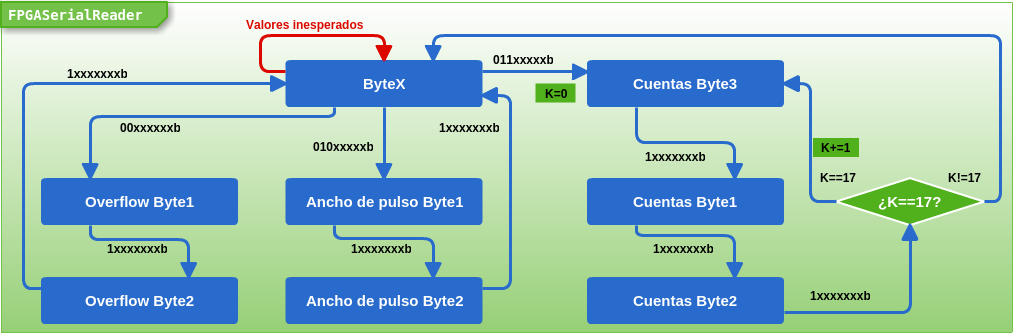
\includegraphics[keepaspectratio, width=1\textwidth]{./img/reader.png}
		\caption{Máquina de Moore. \texttt{FPGASerialReader}.}   
		\label{fig:reader}
	\end{figure}

\section{\texttt{CountsManager}}
	Este es el módulo software encargado de recolectar la información de los demás módulos y guardarla en una base de datos. En la figura
	\ref{fig:soft_adquisición} podemos ver el diagrama que describe el funcionamiento de este. La mayoría de los datos que este módulo maneja son
	generados por los otros módulos software como el \texttt{FPGASerialReader} o el \texttt{SensorsManager}, este tan sólo calcula el valor global
	y las correcciones de este. Finalmente este se encarga de guardar los datos. 
	\subsection{Solicitar cuentas a la FPGA}
		Como vimos en el capítulo \ref{entornoHW} la FPGA tan sólo transmite los datos de las cuentas cuando estas son solicitadas con el
		comando apropiado. Este módulo es el encargado de mandar el comando al principio de cada minuto. La información transmitida por la
		FPGA es procesada por el \texttt{FPGASerialReader} y almacenada en variables compartidas accesibles por el \texttt{CountsManager}.
		Después de mandar el comando apropiado para solicitar las cuentas este Thread se queda esperando hasta que el
		\texttt{FPGASerialReader} le notifique de que las cuentas han sido enviadas y procesadas. Al ser notificado este módulo procede a leer
		de las variables compartidas donde está almacenada la información de las cuentas.
	\subsection{Median Algorithm y Correcciones}
		Como hemos comentado al principio de esta sección este módulo calcula el valor global y una serie de correcciones sobre este. El valor
		global es una representación de las mediciones de todos los tubos, algo como una media. En el capítulo \ref{cap1} explicamos la
		necesidad de este valor, en este vamos a explicar el algoritmo que es utilizado para calcular este valor.
	  	\par 
		El MedianAlgorithm\cite{MedianAlgr} tiene dos entradas, un vector con las cuentas actuales de cada canal y un segundo vector con la
		media de cuentas para cada canal. Este vector con cuentas medias es calculado durante un intervalo temporal en el que la presión
		atmosférica no fluctúa y además esta se corresponde al valor medio de presión para la estación. Además es deseable que durante dicho
		intervalo no ocurran eventos que pueden afectar la cantidad de partículas que llegan al instrumento. Este vector de valores medio es
		especificado  en el archivo de configuración que previamente discutimos por lo que es fácilmente modificable. El algoritmo empieza
		calculando la desviación relativa sobre la media de cada canal, los canales con una desviación grande son descartados. Comparando la
		desviación de los canales restantes seleccionamos el mediano, de aquí el nombre del algoritmo. La desviación relativa del canal
		seleccionado es multiplicada por el sumatorio del vector de cuentas medias. El algoritmo devuelve el valor generado por la
		multiplicación. A continuación presentamos la implementación del algoritmo.
		\begin{lstlisting}[style=myPython]
def medianAlgorithm(self, counts):
   # Calculamos la desviación sobre la media.
   r=[x/z for x,z in zip(counts, self.channel_avg) 
      # Descartamos los canales con desviación grande.
      if z>0 and (x/z)>0.3 and (x/z)<10]
   tet = numpy.median(r)
   s0  = sum(self.channel_avg)
   return s0*tet
		\end{lstlisting}
		\par 
		Una vez calculado el valor global usando el MiedianAlgorithm procedemos a calcular las dos correcciones. La primera es la corrección
		por presión. Como explicamos en el cápitulo \ref{cap1} la presión atmosférica influye en el proceso de adquisición. Para realizar la
		corrección por presión hay dos factores que se toman en cuenta. El primero es la desviación de la presión actual respecto al valor
		medio de presión para la estación. El segundo es el coeficiente de correlación de los tubos respecto a la presión atmosférica. Este
		coeficiente ha sido calculado por el equipo de CALMA, siendo el método utilizado desconocido para el autor de este trabajo. En la
		ecuación \ref{eq:pression} podemos ver como se usan estos dos factores, donde $N_0$ es el valor sin corregir, $N$ el valor corregido,
		$\beta$ el coeficiente de corelación, $P$ la presión actual y $P_0$ la presión media para la estación.
		\begin{equation}\label{eq:pression}
		  N=N_0*exp(\beta*(P-P_0))
		\end{equation}
		La segunda corrección que realizaremos es la corrección por eficiencia. Esta es una corrección muy simple, consiste en aplicar un
		factor multiplicativo a la corrección por presión. Esta corrección se puede ver en la formula \ref{eq:efficiencia}, donde $N_0$ es el
		valor de la corrección por presión, $N$ el valor de la corrección por eficiencia y $\beta$ el factor de corrección. 
		\begin{equation}\label{eq:efficiencia}
		  N=N_0*\beta
		\end{equation}
		Cambios en el entorno de la estación pueden causar cambios en la cantidad de eventos medidos, por ejemplo la construcción cercana de
		un nuevo edificio podría reducir la cantidad de partículas que llegan al instrumento. Una persona que analiza los datos con propósito
		científico puede equívocamente asociar el decremento con algún fenómeno físico, mientras que este es debido a un fenómeno técnico.
		Este problema es solventado con la corrección por eficiencia.   

	\subsection{Base de datos}
		Como ya hemos explicado los datos son guardados en una base de datos para cuya gestión utilizamos Sqlite3. En la base de datos tenemos
		tres tablas que a continuación procedemos a explicar.
	    	\par
		La primera tiene el nombre de \texttt{binTable}, nombre que hemos heredado del NMDB. En esta guardamos la información de las cuentas
		de cada minuto. Junto a las cuentas guardamos la fecha y hora actuales, la lectura del barómetro y la lectura de las fuentes de alta
		tensión.
	    	\par 
		En la segunda tabla llamada CALM\_ori, nombre también heredado por el NMDB, guardamos el valor global y sus correcciones. Junto a
		estos valores también guardamos el valor de la fecha y hora actuales, y en este caso tan sólo guardamos el valor de la presión
		atmosférica.
	    	\par
		En la última tabla guardamos los valores de los anchos de pulsos. Dado al gran número de pulsos que son procesados guardar la
		información de cada uno por separado no es práctico. Para ilustrar el problema pondremos de ejemplo la estación de CALMA donde son
		procesados unos 4500 pulsos cada minuto, siendo esta una de las estaciones con menos eventos por minuto debido a su pequeña latitud.
		Para sobrevenir este problema construimos un histograma que guardamos en la base de datos en forma de cadenas JSON\cite{JSON}. Los
		histogramas son construidos con los datos de diez minutos, intervalo que marca la resolución de los datos de esta tabla.

\section{\texttt{DBUpdater}}
	Este módulo software es el encargado de actualizar el contenido de la base de datos remota. El funcionamiento de este es muy simple y se puede
	ver en la figura \ref{fig:soft_adquisición}. Empieza estableciendo la conexión con la base de datos remota. Si esta se establece procede a leer la
	última entrada en la base de datos remota. Seguidamente el software calcula la diferencia entre las dos bases de datos, para el propósito usa
	la fecha y hora de la entrada leída de la base de datos remota. Finalmente el software selecciona las diferencias entre las dos bases de datos
	y las escribe en la remota. Es entonces cuando la ejecución de este Thread termina. 
	\par
	Si la conexión con la máquina que alberga a la base de datos remota se pierde por un tiempo, cuando esta vuelva a restablecerse el
	\texttt{DBUpdater} sincronizara las dos bases de datos. Eventualmente si las diferencias entre las dos bases de datos son muy grandes la
	sincronización no ocurre de golpe, de esta manera evitamos sobrecargar al sistema. El fallo de la sincronización no es crítico, el Thread
	volverá a ser lanzado el próximo minuto y volverá intentar sincronizar las dos bases de datos.

\section{\texttt{SensorsManager}}
	Este es el módulo software encargado de manejar los sensores, por sensores nos referimos al barómetro, las fuentes de alta tensión o los
	termómetros si están presentes. A este módulo le es pasada la información referente a los sensores del archivo de configuración. De acuerdo
	con esta información este módulo invoca las funciones de configuración necesarias. Una vez realizada esta configuración inicial podemos
	empezar a leer la información de los sensores, para este propósito este módulo exporta tres funciones. A continuación explicaremos estas tres
	funciones.
	\subsection{Presión atmosférica}
		Para leer el valor actual de la presión atmosférica este módulo nos ofrece la función \texttt{read\_pressure}. Si en el archivo de
		configuración hemos especificado que no tenemos barómetro esta función devuelve un \emph{-1}, valor que devuelve en caso de algún
		error. Actualmente son soportados dos tipos de barómetros, el BM35 y el AP1. La lógica para manejar estos dos barómetros
		se encuentra en los archivos \texttt{BM53Driver} y \texttt{AP1Driver} respectivamente. No explicaremos muy a fondo el funcionamiento
		de estos dos, tan sólo destacaremos que el BM35 se comunica mediante un puerto serie y el AP1 mediante tres señales digitales que son
		reloj, \emph{strobe} y datos.
	\subsection{Fuentes de alta tensión}
		En el caso de las fuentes de alta tensión las tenemos de dos tipos, analógicas y digitales. Las digitales transmiten su información
		mediante un puerto serie. Las analógicas mediante una señal analógica entre 0V y 5V, siendo la amplitud de esta señal proporcional a
		la amplitud de la corriente generada por la fuente. La lógica para operar con las fuentes analógicas está en el archivo
		\texttt{HVPSDriver}, la lógica para las fuentes digitales no está implementada porque no hemos podido trabajar con estas.
		Eventualmente si se produce algún error es devuelto el valor de \emph{-1}.
	\subsection{Temperatura}
		Como hemos comentado en muchas estaciones la temperatura ambiente es monitorizada también. Este no es el caso de CALMA, razón por la
		que no hemos escrito ningunos drivers. Sin embargo el código está pensado para poder ser fácilmente ampliado en caso de necesidad. 

\section{Pruebas unitarias}
	Durante la realización de este trabajo hemos escrito una serie de test unitarios\cite{UnitTest}. Los test unitarios son una técnica que
	permite comprobar el funcionamiento correcto de pequeños módulos o funciones. Las pruebas unitarias a diferencia de otras técnicas pueden ser
	usadas desde una etapa muy inicial del proyecto, incluso existen metodologías como \emph{Desarrollo dirigido por pruebas} donde las pruebas
	son escritas primero y después es escrita la función que pasa la prueba. Recalcamos que en este trabajo no hemos seguido esta metodología.
	\par
	Para que las pruebas unitarias sean aplicables es necesario que el código este bien estructurado. Un código con funciones pequeñas donde cada
	función tiene un propósito bien definido es fácil de testear. El simple hecho de poder escribir un test de una función indica que dicha
	función está bien estructurada. Escribir pruebas unitarias conlleva refactorizar el código, haciéndolo mejor.
	\par
	Las pruebas unitarias son muy útiles y es recomendable que estas tengan una gran cobertura, pero no siempre es posible escribir pruebas
	unitarias para todas las funciones. Pongamos como ejemplo una función que lee una entrada desde una base de datos. Aunque la función este bien
	estructurada es difícil testearla por múltiples razones. Por ejemplo el valor devuelto depende de los datos presentes en la base de datos,
	suponiendo que esta está presente y está configurada correctamente. Es difícil escribir pruebas unitarias para este tipo de funciones, razón
	por la que existen las pruebas de integración.
	\par
	Para realizar los test unitarios hemos utilizado \emph{mocks}(objetos simulados). Estos son objetos que simulan el comportamiento de objetos
	reales de una forma controlada. Por ejemplo en nuestra aplicación hemos utilizado un \emph{mock} para simular el comportamiento de los puertos
	serie. Veamos un pequeño ejemplo donde comprobamos la función \texttt{FPGASerialReader.run()}, función que es encargada de interpretar los
	datos que llegan por la UART de pulsos desde la FPGA.
	\begin{lstlisting}[style=myPython]
def test_high_level_pulse(self):
   port=MagicMock()
   port.inWaiting.return_value=1
   # Secuencia de bytes que representan un mensaje de
   # ancho de pulso.
   port.read.side_effect= \
        ReturnSequence([['\x43'],['\x80'],['\xA0']],None)	

   reader=FPGASerialReader(port, None, [], [], [])
   reader.run()
   self.assertEqual(reader.shared_countsFromEvents[3],1)
#------------------------------------------------------
class ReturnSequence(object):
   def __init__(self, return_sequence, expired):
      self.return_sequence = return_sequence
      self.expired = expired
   def __call__(self, *args):
      if 0  < len(self.return_sequence):
         return self.return_sequence.pop(0)
      else:
         return self.expired
	\end{lstlisting}
	\par
	El objeto \texttt{port} es el objeto que representa el puerto como vemos este es un \emph{mock}. La función \texttt{inWaiting} que devuelve el
	número de datos disponibles es configurada para que siempre devuelva \texttt{1}. La función \texttt{read} es configurada para devolver
	múltiples valores en un orden concreto. Seguidamente es creado el objeto cuya función queremos probar pasándole la referencia del mock, una
	vez creado invocamos la función \texttt{run}. Finalmente comprobamos si el atributo \texttt{shared\_countsFromEvents} tiene el valor esperado.
	\par
	En el ejemplo anterior hicimos la comprobación sobre el valor de un atributo con la función \texttt{assertEqual()}. Los \emph{mocks} ofrecen
	aún más funcionalidad, las funciones \texttt{assert\_called\_with()} y \texttt{assert\_has\_calls()} que permiten comprobar las llamadas que
	han sido realizadas sobre los \emph{mocks}.
	\par
	Junto a las pruebas unitarias hemos utilizado la librería \texttt{coverage} que permite medir la cobertura de estas. Una mayor cobertura
	siempre es mejor, pero no debe convertirse en un objetivo principal. Como hemos dicho para ciertas funciones, como las que interactúan con una
	base de datos es difícil concebir una prueba unitaria. En la figura \ref{fig:coverage} presentamos el resumen de cobertura generado por
	\texttt{coverage}. Podemos ver que las pruebas para el \texttt{CountManager} no son muy extensas debido a que este es un módulo que interactúa
	mucho con las bases de datos. Sin embargo podemos ver que la cobertura del \texttt{DBUpdater} es del 100\%, esto es debido a que los test
	escritos para este módulo no son unitarios, esto son más bien test de integración. Durante el proceso de implementación surgió la necesidad de
	estos, razón por la que son incluidos en este trabajo.
	\begin{figure}[h]
		\centering
		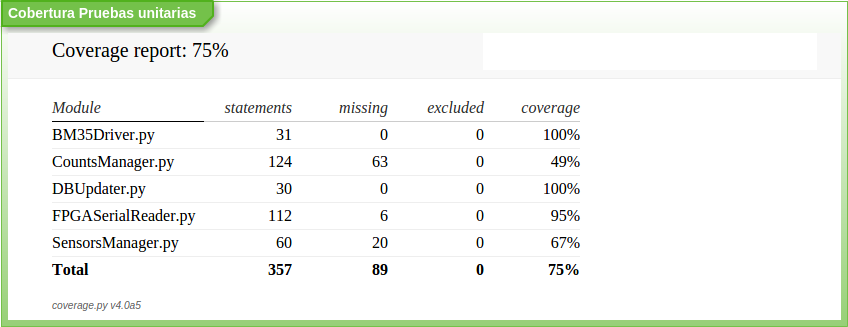
\includegraphics[keepaspectratio, width=1\textwidth]{./img/coverage.png}
		\caption{Cobertura Pruebas unitarias}   
		\label{fig:coverage}
	\end{figure}

\section{Implantación y mantenimiento}
	Como hemos explicado en el capítulo de introducción aparte de implementar el software tenemos como objetivo implantar y realizar el
	mantenimiento de este durante un tiempo. 
	\par
	Implantar el software implica implantar el sistema de adquisición entero. En esta labor obtendremos la ayuda del equipo responsable de la
	estación de CALMA. El sistema tendrá que funcionar conjuntamente al sistema de adquisición ya existente, compartiendo los tubos contadores, el
	barómetros y el resto de elementos necesarios. Para resolver este problema tendremos que realizar una serie de artimañas tanto hardware como
	software. El objetivo principal es desplegar el sistema, pero interferir lo menos posible en el funcionamiento del sistema de adquisición ya
	presente. 
	\par
	Una vez puesto en marcha el nuevo sistema de adquisición nuestra labor será vigilar por el correcto funcionamiento de este. Tendremos que
	localizar y corregir los problemas que se presenten. Finalmente elaboraremos un resumen de esta experiencia. Este resumen será presentado en
	el capítulo \ref{cap_conclusiones}.

\chapter{Herramienta Web. Back End}
\label{backend}

Fijándonos en el diseño preliminar de la figura \ref{fig:herramienta_web_preliminar} podemos ver que nuestra aplicación Web está dividida en
\emph{front-end} y \emph{back-end}. Esta separación entre módulos es una técnica popular en diseño software. El \emph{front-end} es el encargado de
la capa de presentación, sobre este hablaremos más en el próximo capítulo. En este capítulo nos centraremos en explicar el \emph{back-end}. Este es el
encargado de procesar las peticiones provenientes del \emph{front-end} y devolver le a este la información solicitada. 
\par
El \emph{back-end} es implementado en PHP\cite{PHP}. Este es un lenguaje diseñado para desarrollo Web y además es una elección muy popular. 
Hemos utilizado ZendFramework\cite{ZF}, este es un framework orientado al desarrollo de aplicaciones Web. Junto al framework hemos utilizado
Apigility\cite{Apigility}, herramienta que simplifica la creación y mantenimiento de APIs.
\par
El \emph{back-end} tiene un enfoque RPC (llama de procedimiento remoto). Este módulo exportara un conjunto de procedimientos que pueden ser invocados
por el \emph{front-end}. Estos procedimientos realizan tareas específicas sobre un recurso concreto. A la largo de este trabajo nos referiremos
a estos procedimientos como \emph{servicios RPC}.
\par
Un aspecto oportuno destacar es que los servicios RPC son sin estado. Esto quiere decir que la respuesta a un procedimiento no es influenciada por
eventos anteriores, esta tan solo depende de los parámetros proporcionados.
\par
Si nos volvemos a fijar en la figura \ref{fig:herramienta_web_preliminar} podemos ver que en el \emph{back-end} existe la separación entre 
\emph{Modelo} y \emph{Controlador}. Esta separación sigue el patrón de diseño MVC\cite{MVCWiki}. Podemos ver que el componente de \emph{Vista} no
existe, en este caso el \emph{front-end} es nuestro componente de \emph{Vista}. Todos los servicios RPC tienen su parte proporcional de
\emph{Modelo} y \emph{Controlador}. La parte de \emph{Modelo} es la encargada de gestionar la información contenida en la base de datos. La parte de
\emph{Controllador} la encargada de gestionar los mensajes de petición y respuesta.
\par
En este capítulo procederemos a explicar los servicios RPC, pero primero explicaremos algunos aspectos técnicos como la base de datos o el ZendFramework.
\section{Protocolo de comunicación}
	Hemos explicado que entre el \emph{back-end} y \emph{front-end} existe una comunicación, para la que hemos elegido un enfoque RPC. En este
	apartado nos centraremos en un aspecto más técnico de esta comunicación. 
	\par
	Siendo la aplicación que desarrollamos una aplicación Web es de esperar que el protocolo utilizado para la comunicación entre los dos módulos
	sea \emph{HTTP}. En este protocolo se puede diferenciar entre dos tipos de mensajes, mensajes de petición y de respuesta. En nuestra
	aplicación el \emph{front-end} enviara mensajes de petición al \emph{back-end}. Los mensajes de petición especifican un campo URL, este campo
	es muy importante porque especifica el servicio RPC que se desea invocar. A la URL también son anexados los parámetros necesarios para el
	procedimiento especificado. Los mensajes de respuesta serán discutidos en el capítulo dedicado el \emph{front-end}.
\section{ZendFramework y Apigility}
	Para la realización de este trabajo hemos utilizado ZendFramework, este es un framework orientado al desarrollo de aplicaciones y servicios Web.
	Basado en PHP 5.3+ el framework sigue un diseño orientado a objetos. Esta enfocado para crear aplicaciones siguiendo el patrón MVC. Ofrece
	abstracciones para las bases de datos, autenticación y validación de parámetros. El framework también disfruta de una amplia comunidad de 
	usuarios. Todas estas ventajas nombradas anteriormente son la razón para elegir este framework en nuestro trabajo.
	\par
 	Para  los principiantes el framework ofrece la aplicación esqueleto. Esta aplicación consiste del código mínimo necesario para construir una
	aplicación usando ZendFramework, no tiene ninguna funcionalidad y esta pensada para ser extendida. En este trabajo hemos empezado con esta
	aplicación esqueleto.
  	\par
	Apigility es una herramienta creada por el equipo responsable de ZendFramework. La herramienta puede utilizarse sin necesidad del framework,
	sin embargo esta se integra muy bien con este. La herramienta facilita la creación y mantenimiento de aplicaciones Web. En nuestro caso la
	herramienta nos ha ayudado a crear los servicios RPC de nuestra aplicación. La aplicación ofrece un entorno gráfico accesible desde un navegador
	Web. El uso de la aplicación es muy fácil e intuitivo.
\section{Bases de datos}
	Tal y como hemos explicado al principio del capítulo la función del \emph{back-end} es  procesar las peticiones del \emph{front-end} y
	responderle con la información solicitada. Esta información es guardada en dos bases de datos. Para la gestión de las bases de datos
	utilizamos MySql\cite{MySql}. ZendFramework ofrece abstracciones para las bases de datos, esto facilita el trabajo con estas. En la
	figura \ref{fig:tablas} podemos ver el esquema de las tablas con las que vamos a trabajar.
	\par
	En la tabla \texttt{binTable} guardamos la información de las cuentas de cada canal. Junto a esa información guardamos las lecturas del
	barómetro, las fuentes de alta tensión y la fecha y hora actuales. La resolución de los datos es de un minuto.
	\par
	En la tabla \texttt{CALM\_ori} guardamos el valor global y  las correcciones sobre este. La lectura de presión atmosférica también es guardada.
	La resolución de estos datos es también de un minuto.
	\par
	En la tabla \texttt{CALM\_rev} guardamos la revisión de los datos de \texttt{CALM\_ori}. Vemos que la tabla tiene el mismo esquema con dos
	campos adicionales. En estos dos campos se guardan la fecha de última modificación y la versión. Los datos en esta tabla son introducidos por
	un operario. Cuando este encuentra un dato corrupto en los datos originales, puede crear una entrada en esta base de datos para señalarlo.
	\par
	La tabla \texttt{binTable} es contenida en una base de datos con el nombre \texttt{nmdadb}. Las tablas \texttt{CALM\_ori} y \texttt{CALM\_rev}
	son contenidas en otra base de datos con el nombre \texttt{nmdb}. Esta separación es algo que hemos heredado del NMDB, detrás no hay un motivo
	justificado. En este documento hablaremos a nivel de tablas, muchas veces sin tener en cuenta la separación en diferentes bases de datos. En
	este punto destacamos esta separación para no crear confusión al lector a la hora de contrastar el código fuente con este documento. 
	\begin{figure}[h]
		\centering
		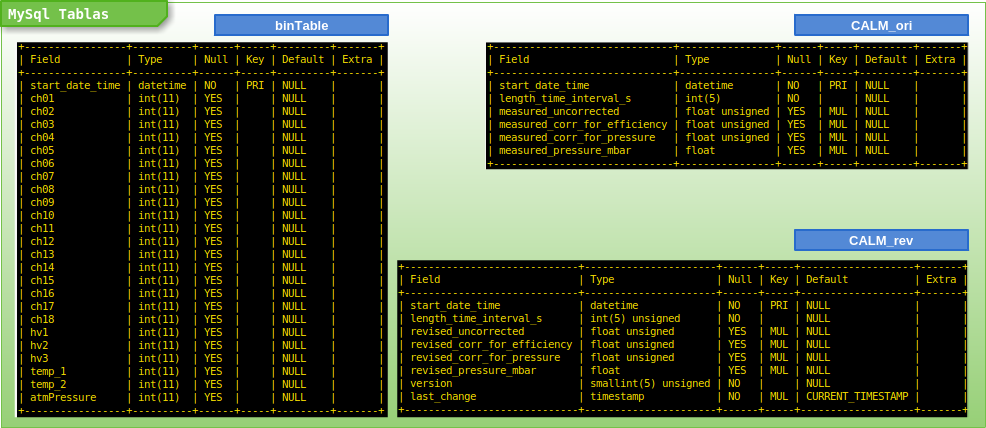
\includegraphics[keepaspectratio, width=1\textwidth]{./img/tablas.png}
		\caption{Esquema de las tablas.}
		\label{fig:tablas}
	\end{figure}
\section{Servicios RPC}
	Es esta sección procederemos a explicar uno a uno los servicios RPC que nuestro \emph{back-end} ofrece. Para cada servicio RPC explicaremos la
	funcionalidad, la URL que le identifica, los parámetros aceptados, la query SQL utilizada y el propósito de este.
	\subsection{\texttt{nmdbOriginalRaw}}
		Este servicio RPC devuelve los datos de la tabla \texttt{CALM\_ori} en un intervalo determinado. Tal y como explicamos en esta
		tabla son guardados los datos globales de la estación, las dos correcciones de estos y los valores de presión atmosférica. Este servicio
		devuelve los datos tal y como están en la base de datos. 
	  	\par
	  	La URL que identifica a este servicio tiene el siguiente formato.
	  		\begin{center} \texttt{/nmdb/original/raw[/:start][/:finish]}  \end{center} 
		Como vemos el servicio acepta dos parámetros, \texttt{start} y \texttt{finish}. Los parámetros delimitan el intervalo de datos
		devueltos.
		\par
		A continuación podemos ver la query SQL utilizada para obtener los datos, dado a la simplicidad de esta no procederemos a discutirla
		mas a fondo.
	  		\begin{center} \texttt{"SELECT * FROM CALM\_ori 
			  		\\	WHERE start\_date\_time BETWEEN \cc".\$start."\cc AND \cc".\$finish"\cc"}
			\end{center} 
		Los datos devueltos por este servicio RPC son utilizados para construir un gráfico lineal.
	\subsection{\texttt{nmdbOriginalGroup}}
		Este servicio RPC es similar al anteriormente descrito, devuelve los datos de la tabla \texttt{CALM\_ori} en un intervalo determinado.
		La diferencia de este servicio es que no devuelve los datos en crudo. Este junta los datos en grupos y devuelve los valores para
		cada grupo. 
		\par
		A continuación podemos ver el formato de la URL que identifica a este servicio.
			\begin{center} \texttt{/nmdb/original/group[/:start][/:finish][/:points]}  \end{center} 
		Los dos parámetros \texttt{start} y \texttt{finish} al igual que en el servicio anterior delimitan el intervalo de datos. En este
		servicio estos dos parámetros pueden tener el valor \texttt{all}, de ser así son utilizados todos los datos presentes en la base de
		datos. El parámetro \texttt{points} especifica en número de grupo en los que serán agrupados nuestros datos.
		Seguidamente podemos ver parte de la query SQL utilizada en este servicio. Esta parte es la encargada de agrupar nuestros datos.
			\begin{center} \texttt{"(SELECT CALM\_ori.*,
			  		\\	(UNIX\_TIMESTAMP(start\_date\_time) DIV (".\$interval.")) AS timekey  
				      	\\	FROM CALM\_ori WHERE start\_date\_time BETWEEN \cc".\$start."\cc AND \cc".\$finish."\cc)AS t1  GROUP BY timekey"}
			\end{center} 
		Como podemos ver son seleccionados los datos presentes en el intervalo definido por \texttt{\$start} y \texttt{\$finish}. Junto a los datos
		presentes en la tabla \texttt{CALM\_ori} es calculado el campo \texttt{timekey}, este campo es el utilizado para formar los grupos. El 
		\texttt{timekey} es calculado utilizando el valor de la variable \texttt{\$interval}, variable que define el intervalo de los grupos
		y es calculada de la siguiente forma.
			\begin{center} \texttt{\$interval =round((\$finish-\$start)/(\$points));}  \end{center} 
		Una vez formados los grupos para cada campo es calculado el máximo, mínimo, \emph{open} y \emph{close}. El \emph{open} y \emph{close}
		son la media más la desviación típica y la media menos la desviación típica respectivamente. Estos cuatro valores son calculados para el
		valor global, la corrección por presión y la corrección por eficiencia. Para la presión atmosférica tan solo es calculado el valor
		medio. Estos datos son utilizados para construir un gráfico \emph{Candlestick}, sobre este tipo de gráfico hablaremos en el
		siguiente capítulo dedicado al \emph{front-end}.
	\subsection{\texttt{nmdbRevisedRaw}}
		Este servicio es muy similar al \texttt{nmdbOriginalRaw}, la diferencia esta en que este devuelve los datos revisados. Para este
		propósito son utilizados los datos de las tablas \texttt{CALM\_ori} y \texttt{CALM\_rev}. La URL utilizada para identificar este
		servicio tiene el siguiente formato.
	  		\begin{center} \texttt{/nmdb/revised/raw[/:start][/:finish]}  \end{center} 
		Los dos parámetros aceptados delimitan el intervalo de datos.
		\par
		En la tabla \texttt{CALM\_rev} son guardados los datos revisados, pero no son guardados todos, tan solo las entradas que han sido modificadas.
		Por esta razón este servicio también hace uso de \texttt{CALM\_ori} para devolvernos la información completa. A continuación podemos
		ver parte de la query SQL utilizada para obtener los datos revisados.
			\begin{center} \texttt{"SELECT ori.start\_date\_time,
			  		\\	CASE WHEN rev.start\_date\_time IS NULL THEN ori.measured\_uncorrected ELSE rev.revised\_uncorrected END AS uncorrected 
					\\	FROM CALM\_ori ori LEFT JOIN CALM\_rev rev ON ori.start\_date\_time = rev.start\_date\_time"}
			\end{center} 
		La query empieza haciendo un \texttt{LEFT JOIN} entre las tablas \texttt{CALM\_ori} y \texttt{CALM\_rev} sobre los campos de
		\texttt{start\_date\_time}. El \texttt{LEFT JOIN} devuelve todas las entradas de \texttt{CALM\_ori}, con las entradas coincidentes de
		\texttt{CALM\_rev}. La parte correspondiente al \texttt{CALM\_rev} es dejada a \texttt{NULL} si no existe coincidencia. A partir de la
		tabla temporal creada por el \texttt{LEFT JOIN} seleccionamos los datos del \texttt{CALM\_rev} si estos están presentes, sino nos
		quedamos con lo datos del \texttt{CALM\_ori}. Los datos devueltos por este servicio serán utilizados para crear un gráfico lineal.
	\subsection{\texttt{nmdbRevisedGroup}}
		Este servicio es muy similar al {\texttt{nmdbOriginalGroup}, pero este hace uso de los datos revisados. La URL que identifica este
		servicio tiene el siguiente formato.
			\begin{center} \texttt{/nmdb/revised/group[/:start][/:finish][/:points]}  \end{center}
		Lo parámetros \texttt{start} y \texttt{finish} delimitan el intervalo de datos. Eventualmente estos dos parámetros pueden tener el
		valor de \texttt{all}, de esta manera son usados todos los datos presentes en la base de datos. El tercer parámetro, \texttt{points},
		especifica el número de grupos en los que queremos agrupar nuestros datos.
		\par
		Para recolectar los datos necesarios la query utilizada es una combinación de las queries utilizadas en los servicios
		\texttt{nmdbOriginalGroup} y \texttt{nmdbRevisedRaw}. Primero realiza un \texttt{LEFT JOIN} entre las tablas \texttt{CALM\_ori} 
		y \texttt{CALM\_rev} para obtener el conjunto de datos revisados. Seguidamente agrupa los datos de este conjunto y para cada grupo
		calcula los valores máximo, mínimo, \emph{open} y \emph{close}. Estos datos son utilizados para construir un gráfico \emph{Candlestick}.

\chapter{Herramienta Web. \emph{Front-End}}
\label{frontend}
Nuestra aplicación Web esta dividida en \emph{back-end} y \emph{front-end}. En el capítulo anterior se describió el \emph{back-end}. El propósito de
este capítulo es describir el \emph{front-end}. El \emph{front-end} es el encargado de la capa de presentación.
\par
El \emph{front-end} es implementado en JavaScript\cite{JavaScript}. Este es un lenguaje de programación soportado por la mayoría de navegadores Web,
nos permite dotar de funcionalidad extendida a nuestras páginas Web. Actualmente el uso de este lenguaje esta tan extendido y avanzado que permite
crear aplicaciones enteras para navegadores Web. Existen múltiples frameworks escritos en JavaScript que facilitan la creación de aplicaciones Web. En
este trabajo vamos a utilizar dos, Sencha ExtJs\cite{ExtJs} y HighStock\cite{HighStock}.
\par
Sencha ExtJs es un framework orientado a la creación de aplicaciones Web interactivas. Debido al gran abanico de funcionalidades que este framework
presenta, podemos decir que este es de propósito general. Este ofrece abstracciones para gestionar nuestros datos, arquitectura MVC, componentes
gráficos de control y otros.
\par
HighStock es un framewrok con un propósito específico. Este está orientado a facilitar la creación de gráficos. El framework es muy eficiente, esto
reduce la carga computacional de nuestra aplicación. Los gráficos generados por este son altamente interactivos, permiten ocultar series, navegar,
realizar zoom y mucho más
\par
Como podemos ver en la figura \ref{fig:frontend} nuestro \emph{front-end} esta basado en el patrón de diseño 
\emph{modelo-vista-controlador}\cite{MVCWiki}.
\begin{figure}[h]
	\centering
	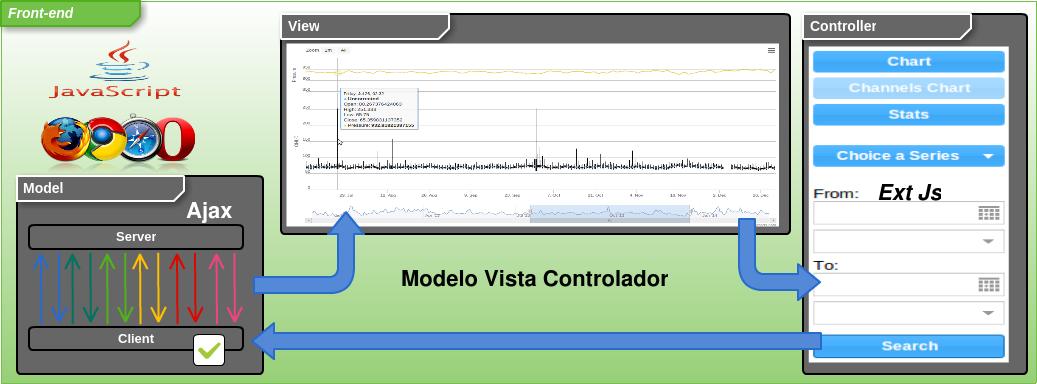
\includegraphics[keepaspectratio, width=1\textwidth]{./img/frontend.png}
	\caption{\emph{Front-end}. Patrón MVC.}   
	\label{fig:frontend}
\end{figure}
\section{Sencha ExtJs}
	El propósito de esta sección es explicar alguno de los aspectos básicos del framework. Empezaremos explicando como crear una aplicación básica
	basándonos en ExtJs. En la mayoría de los casos existe un solo documento HTML\cite{HTML} que contiene toda la aplicación. En este documento
	tenemos que cargar dos \emph{scripts} de la siguiente forma.
 	%<Script1>
 	%<Script2>
 	El primer \emph{script} contiene el framework que queremos utilizar. Es conveniente destacar que esta es una versión concebida para el proceso
	de desarrollo. Para la versión final es conveniente usar el \texttt{ext-all.js}.
 	\par
 	El segundo \emph{script} es el que contiene la lógica de nuestra aplicación. A continuación podemos ver el código mínimo para crear una
	aplicación. El código presentado será explicado a fondo.
 	%<Código>
 	En la primera línea hacemos uso del singletone \texttt{Ext}. Este es un objeto que encapsula todas las clases, métodos y singletones
	proporcionados por el framework. La función utilizado \texttt{Ext.application} carga e inicializa una instancia de la clase
	\texttt{Ext.app.Application}. Esta clase representa una aplicación ExtJs single page. La llamada a esta función crea la variable global
	\texttt{MyApp}, que debe contener todas las clases e instancias de nuestra aplicación.
 	\par
 	En la segunda línea declaramos el nombre de nuestra aplicación. Seguidamente definimos la función \texttt{launch}. Esta es la función que debe
	lanzar  nuestra aplicación. La primera función invocada es \texttt{Ext.create} que crear una instancia de la clase proporcionada, en este caso
	\texttt{Ext.container.Viewport}. \texttt{Viewport} es un \emph{contenedor} que representa el área de aplicación y puede haber tan solo uno por
	aplicación. 
 	\par
 	La interfaz de usuario en una aplicación ExtJs es compuesta por \emph{componentes}. Un \emph{contenedor} es un \emph{componente} especial que
	contiene otros \emph{componentes}. En la figura \ref{fds} podemos ver un ejemplo que ilustra esta jerarquía.
 	%<The figure that must be done.>
 	\par
 	El \texttt{Viewport} es el \emph{contenedor} que contiene todos los demás \emph{componentes} de nuestra aplicación. Los \emph{compenentes} de
	un \emph{contenedor} se especifican en el campo \texttt{items} que es una lista. En el ejemplo presentado tan solo tenemos un 
	\emph{conponente}, pero pueden ser añadidos más.
 	\par
 	Fijándonos en el código de ejemplo podemos ver antes de definir el campo \texttt{items} definimos el campo \texttt{layout}. El \texttt{layout}
	especifica la forma en la que se posicionaran y ajustaran los \emph{componetes} hijos. En este caso el \texttt{layout} especificado es 
	\texttt{\cc fit\cc} en el que un solo hijo ocupa todo el espacio del padre. 

\section{\emph{Modelo}}
	El \emph{modelo} es el encargado de manejar los datos de una aplicación. En el caso del \emph{front-end} los datos de la aplicación deben ser
	servidos por el \emph{back-end}. El \emph{modelo} es el encargado de realizar la comunicación con el \emph{back-end}. 
	\par
	Tal y como especificamos en el  capítulo anterior el protocolo para la comunicación entre los dos módulos es \emph{HTTP}. Nuestro
	\emph{front-end} es el que empieza la comunicación enviando un mensaje de petición y el \emph{back-end} responde a esa peticion con un mensaje
	de respuesta. El \emph{modelo} es el encargado de construir y enviar los mensajes de petición y después interpretar los mensajes de respuesta.
	\par
	Para dotar el \emph{modelo} de la funcionalidad necesaria vamos a ayudarnos de las facilidades que nos ofrece ExtJs, concretamente vamos a
	utilizar el singletone \texttt{Ext.Ajax}. Ajax\cite{AjaxWiki} es una técnica de desarrollo Web donde cliente y servidor mantienen una
	comunicación asíncrona en segundo plano. \texttt{Ext.Ajax} es un singletone de la clase \texttt{Ext.data.Connection}, clase que encapsula la
	lógica necesaria para realizar una comunicación Ajax. 
	\par
	Concretamente vamos a hacer uso de la función \texttt{Ext.data.Connection.request}. Esta función envía una petición \emph{HTTP} a un servidor
	remoto. La función acepta un solo parámetro que es un objeto cuyas propiedades definen el comportamiento de la función. Las propiedades de las
	que nosotros haremos uso están detalladas a continuación. 
	\begin{itemize}
  		\item	\texttt{url}. 	La URL a la que enviaremos la petición. En nuestro caso \emph{back-end} y \emph{front-end} estarán albergados en
		  	el mismo \emph{host}. Esto nos permite no especificar el \emph{host}, la petición se hará al \emph{host} utilizado para cargar
			la aplicación. En la URL tan solo tendremos que especificar el servicio deseado y los parámetros que acompañan a este.
			Seguidamente presentamos un ejemplo del valor que puede tomar el campo \texttt{url}.
    				\begin{center} \texttt{url: \cc/nmdadb/cannel/stats/default/default\cc}  \end{center}
		\item	\texttt{method}. El método que especifica nuestro mensaje de petición. Los mensajes \emph{HTTP} de petición pueden especificar
		  	un método. Si este campo es dejado vacío el método utilizado será \texttt{GET}. La mayoría de los servicios ofrecidos por el
			\emph{back-end} aceptan un método \texttt{GET}, pero el servicio \texttt{nmdbMarkNull} acepta un método \texttt{POST}.
		\item	\texttt{success}. La función a ser llamada al completar exitosamente la petición. Esta función a su vez acepta como parámetro
		  	\texttt{response}. Este parámetro contiene los datos del mensaje de respuesta.
		\item	\texttt{failure}. La función a ser llamada al completar sin éxito la petición. Esta función también acepta el parámetro
		  	\texttt{response} que podemos utilizar para identificar la causa del fallo.
		\item	\texttt{timeout}. El numero de milisegundos en los que el \emph{back-end} debe responder. Si el tiempo expira la solicitud se
		  	considera como fallida. 
	\end{itemize}
	Más allá de \emph{Ext.data.Connection} el framework ofrece abstracciones de un nivel superior. La clase \emph{Ext.data.Model} es una
	representación de un objeto utilizado por nuestra aplicación. Estos modelos son usados por la clase \emph{Ext.data.Store}, que encapsula
	instancias de un modelo. La clase \emph{Ext.data.Store} también hace uso del \emph{Ext.data.proxy.Proxy}, abstracción que permite cargar y
	guardad datos de un modelo. 
	\par
	Estas abstracciones son muy útiles, pero algo complejas. Al no estar acostumbrado a trabajar con ellas el autor de este trabajo ha preferido
	utilizarlas lo menos posible. Por esta razón la mayoría de los datos se manejan usando el \texttt{Ext.data.Connection}, hemos utilizado el
	\texttt{Ext.data.Store} en casos muy específicos.

\chapter{Conclusiones y trabajos futuros}
\label{cap_conclusiones}

\section{Conclusiones}
\section{Trabajos futuros}
	\subsection{Debian en la BeagleBone Black}
	Para realizar el software de adquisición hemos utilizado Angstrom, la distribución Linux que venía por defecto con la BeagleBone Black.
	Angstrom es una distribución muy ligera y adecuada, pero la comunidad existente es muy pequeña. Nos hemos propuesto como trabajo futuro
	cambiar de la Angstrom a alguna distribución derivada de Debian. Nuestro caso no es algo aislado sino parte de una movimiento mayor, gran
	parte de los usuarios  de BeagleBone Black instalan Debians en sus placas. El fabricante de las placas también anuncio que en un futuro las
	placas llevaran Debian por defecto. Como hemos comentado la razón detrás de esta elección es la comunidad de usuarios. Siendo esta mayor es
	mucho más fácil encontrar información o ayuda. Al hacer este cambio también tendríamos que realizar algunos cambios en nuestro software,
	adaptarlo para el nuevo entorno.
	\subsection{Script de configuración para el software de adquisición}
	Todo el proceso de configuración para implantar el software está reflejado en el archivo \emph{Readme}. Los pasos recogidos en el archivo
	podrían automatizarse, podríamos crear un script que ejecutara todos los comandos necesarios. De esta manera para implantar el software tan
	solo haría falta clonar el repositorio remoto y ejecutar el script. Este script se crearía después de realizar el cambio de distribución a
	Debian.
	\subsection{Watchdog}
	Otro aspecto que podríamos mejorar del software de adquisición es el Watchdog. Tal y como se explicó en el capítulo \ref{cap2} el Watchdog que esta
	implementado actualmente es muy simple. Este tan solo comprueba que el sistema operativo no se quede bloqueado. Si recordamos la función del
	Watchdog es detectar malfuncionamientos y reiniciar el sistema al detectar uno. Que el sistema operativo se quede bloqueado es un
	malfuncionamiento, pero existe otro que también queremos evitar. La función del software es que los datos generados por el resto del sistema
	acaben en una base de datos, que no se generen datos es un malfuncionamiento que queremos evitar. Podremos detectar este problema mirando en
	la base de datos. Ante la presencia de nuevos datos el software tendría que reiniciar el contador del Watchdog y si no están presentes nuevos
	datos el software tendría que no reiniciar el contador. De esta forma si no se generan nuevos datos por el sistema, el software sera
	reiniciado. 
	\subsection{Servicios RPC para el \emph{back-end}}
	Tal y como explicamos en el capítulo dedicado al \emph{back-end} de nuestra herramienta, hemos dado un enfoque REST\cite{Rest} a este.  A lo
	largo de la implementación el autor de este trabajo se ha dado cuenta de que REST no es el mejor enfoque que hayamos podido utilizar. En su
	mayoría nuestros recursos tan solo permitían un solo método. Es aquí donde rompemos con los que establece REST, tener una serie de recursos
	sobre los que podemos aplicar diferentes métodos. 
	\par
	Existe otra técnica llamada RPC que se ajusta mejor a nuestro problema. A diferencia que REST no tenemos recursos con sus métodos, tenemos tan
	solo métodos. Al igual que los recursos estos métodos tienen una URL asociada para identificarlos. Los métodos nos permiten realizar
	operaciones  muy específicas como pueden ser el leer un registro, actualizarlo o borrarlo.




%Incluyo la bibliografía
\addcontentsline{toc}{chapter}{Referencias bibliográficas}
%\let\antiguaLM\leftmark
%\let\antiguaRM\rightmark
%\renewcommand\leftmark{}
\nocite{*}
\bibliographystyle{plain}
\bibliography{Bibliografia}

%Acronyms
\newpage
\printglossary[type=\acronymtype]
\addcontentsline{toc}{chapter}{Acrónimos}
\end{document}
